%%% Generated by SAPlugin v6.0 on Sun Nov 28 22:49:47 CET 2021

\documentclass[english]{sareport}
\newcommand\tab[1][1cm]{\hspace*{#1}}

\usepackage{caption}
\usepackage{rotating}
\usepackage{pdflscape}
\usepackage[colorlinks, linkcolor=black, citecolor=black, urlcolor=black]{hyperref}
\usepackage[sort]{cleveref}
\usetikzlibrary{arrows}

\graphicspath{{./images/}}

% \addAuthor firstname lastname studentnumber
\addAuthor{FirstName3}{LastName3}{r000000}
\addAuthor{FirstName1}{A LastName1}{m000000}
\addAuthor{FirstName2}{B LastName2}{s000000}

%\academicyear{20xx--20xx}

\casename{Document Processing Service (DocProc)}
%\phasenumber{Part 3} % TODO: enter Part 2 or Part 3 as needed
\phasename{Architectural extension}

\newcommand{\inlinetodo}[1]{{\color{red} \textbf{TODO:} #1}}

% EXPORT CMDS
% \texttt layout modifications

\newcommand*\vpejustify{%
	\fontdimen2\font=0.4em%
	\fontdimen3\font=0.8em%
	\fontdimen4\font=0.1em%
	\fontdimen7\font=1.0em%
	\hyphenchar\font=`\-\relax%
}
\newcommand{\vpett}[1]{\vpejustify{\texttt{#1}}}

% item labels
\makeatletter
\def\vpeitemlabel#1#2{\begingroup
	#2%
	\def\@currentlabel{#2}%
	\phantomsection\label{#1}\endgroup
}
\makeatother

% vpe operation
\newcommand{\vpeoperation}[1]{#1}

% vpe data type
\newcommand{\vpedatatype}[2]{\vpeitemlabel{#1}{\textbf{\textsf{#2}}}}

% vpe exception
\newcommand{\vpeexception}[2]{\vpeitemlabel{#1}{\textsl{#2}}}

\newcommand{\iconcomponent}{%
	\begin{tikzpicture}[scale=0.3,thin,baseline=-0.05ex]
	\draw (0,0) rectangle (0.4, 0.6);
	\draw [fill=white] (-0.1,0.40) rectangle +(0.25, 0.1);
	\draw [fill=white] (-0.1,0.22) rectangle +(0.25, 0.1);	
	\end{tikzpicture}%
}
\newcommand{\iconprovided}{%
	\begin{tikzpicture}[scale=0.25,thin,baseline=-0.25ex]
	\draw (0.60,0.25) circle [radius=0.25];
	\draw (0, 0.25) -- (0.35, 0.25);
	\end{tikzpicture}%
}
\newcommand{\iconrequired}{%
	\begin{tikzpicture}[scale=0.25,thin,baseline=-0.25ex]
	\draw (0.60,0) arc (270:90:0.25);
	\draw (0, 0.25) -- (0.35, 0.25);
	\end{tikzpicture}%
}
\newcommand{\iconinher}{%
	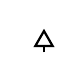
\begin{tikzpicture}[scale=0.3,thick,baseline=-0.5ex]
	\node (0,0) {};
	\draw[-open triangle 60] (.3,-.4) -- (.3, .6);
	\node (.9,0) {};
	\end{tikzpicture}%
}
%  END EXPORT CMDS

\begin{document}
\maketitle

\tableofcontents
% the following two command are necessary for obtaining the mini list of figures in the cs-view, decomposition view, deployment view and scenarios chapters
\dominilof
\fakelistoffigures

% the rationale
%%% Generated by SAPlugin v6.0 on Sun Nov 28 22:49:47 CET 2021

% (optional)
\chapter{Introduction}\label{sec:introduction}


\chapter{QAS Decisions}\label{sec:decisions}


% (optional)
\chapter{Other decisions}\label{sec:otherdecisions}



\chapter{Discussion}\label{sec:discussion}

\appendix

% included tex file contains chapter commands
%%% WARNING %%%
%%% This file was automatically generated by SAPlugin,
%%% and will be overwritten next time.

% macro for maximum width and height
\makeatletter\def\maxwidth#1{\ifdim\Gin@nat@width>#1 #1\else\Gin@nat@width\fi}\makeatother
\makeatletter\def\maxheight#1{\ifdim\Gin@nat@height>#1 #1\else\Gin@nat@height\fi}\makeatother


\graphicspath{appendices/architecture/images/}
%%%%%%%%%%%%%%%%%%%%%%%%%%%%%%%%%%%%%%%%%%%%%%%%%%%%
%%% CS
%%%%%%%%%%%%%%%%%%%%%%%%%%%%%%%%%%%%%%%%%%%%%%%%%%%%
\chapter{Client-server view (UML Component Diagram)}
\minilof{}






%%% DataAnonymizer Component Diagram (656.0x257.0)

\begin{figure}[!htp]
  \centering
  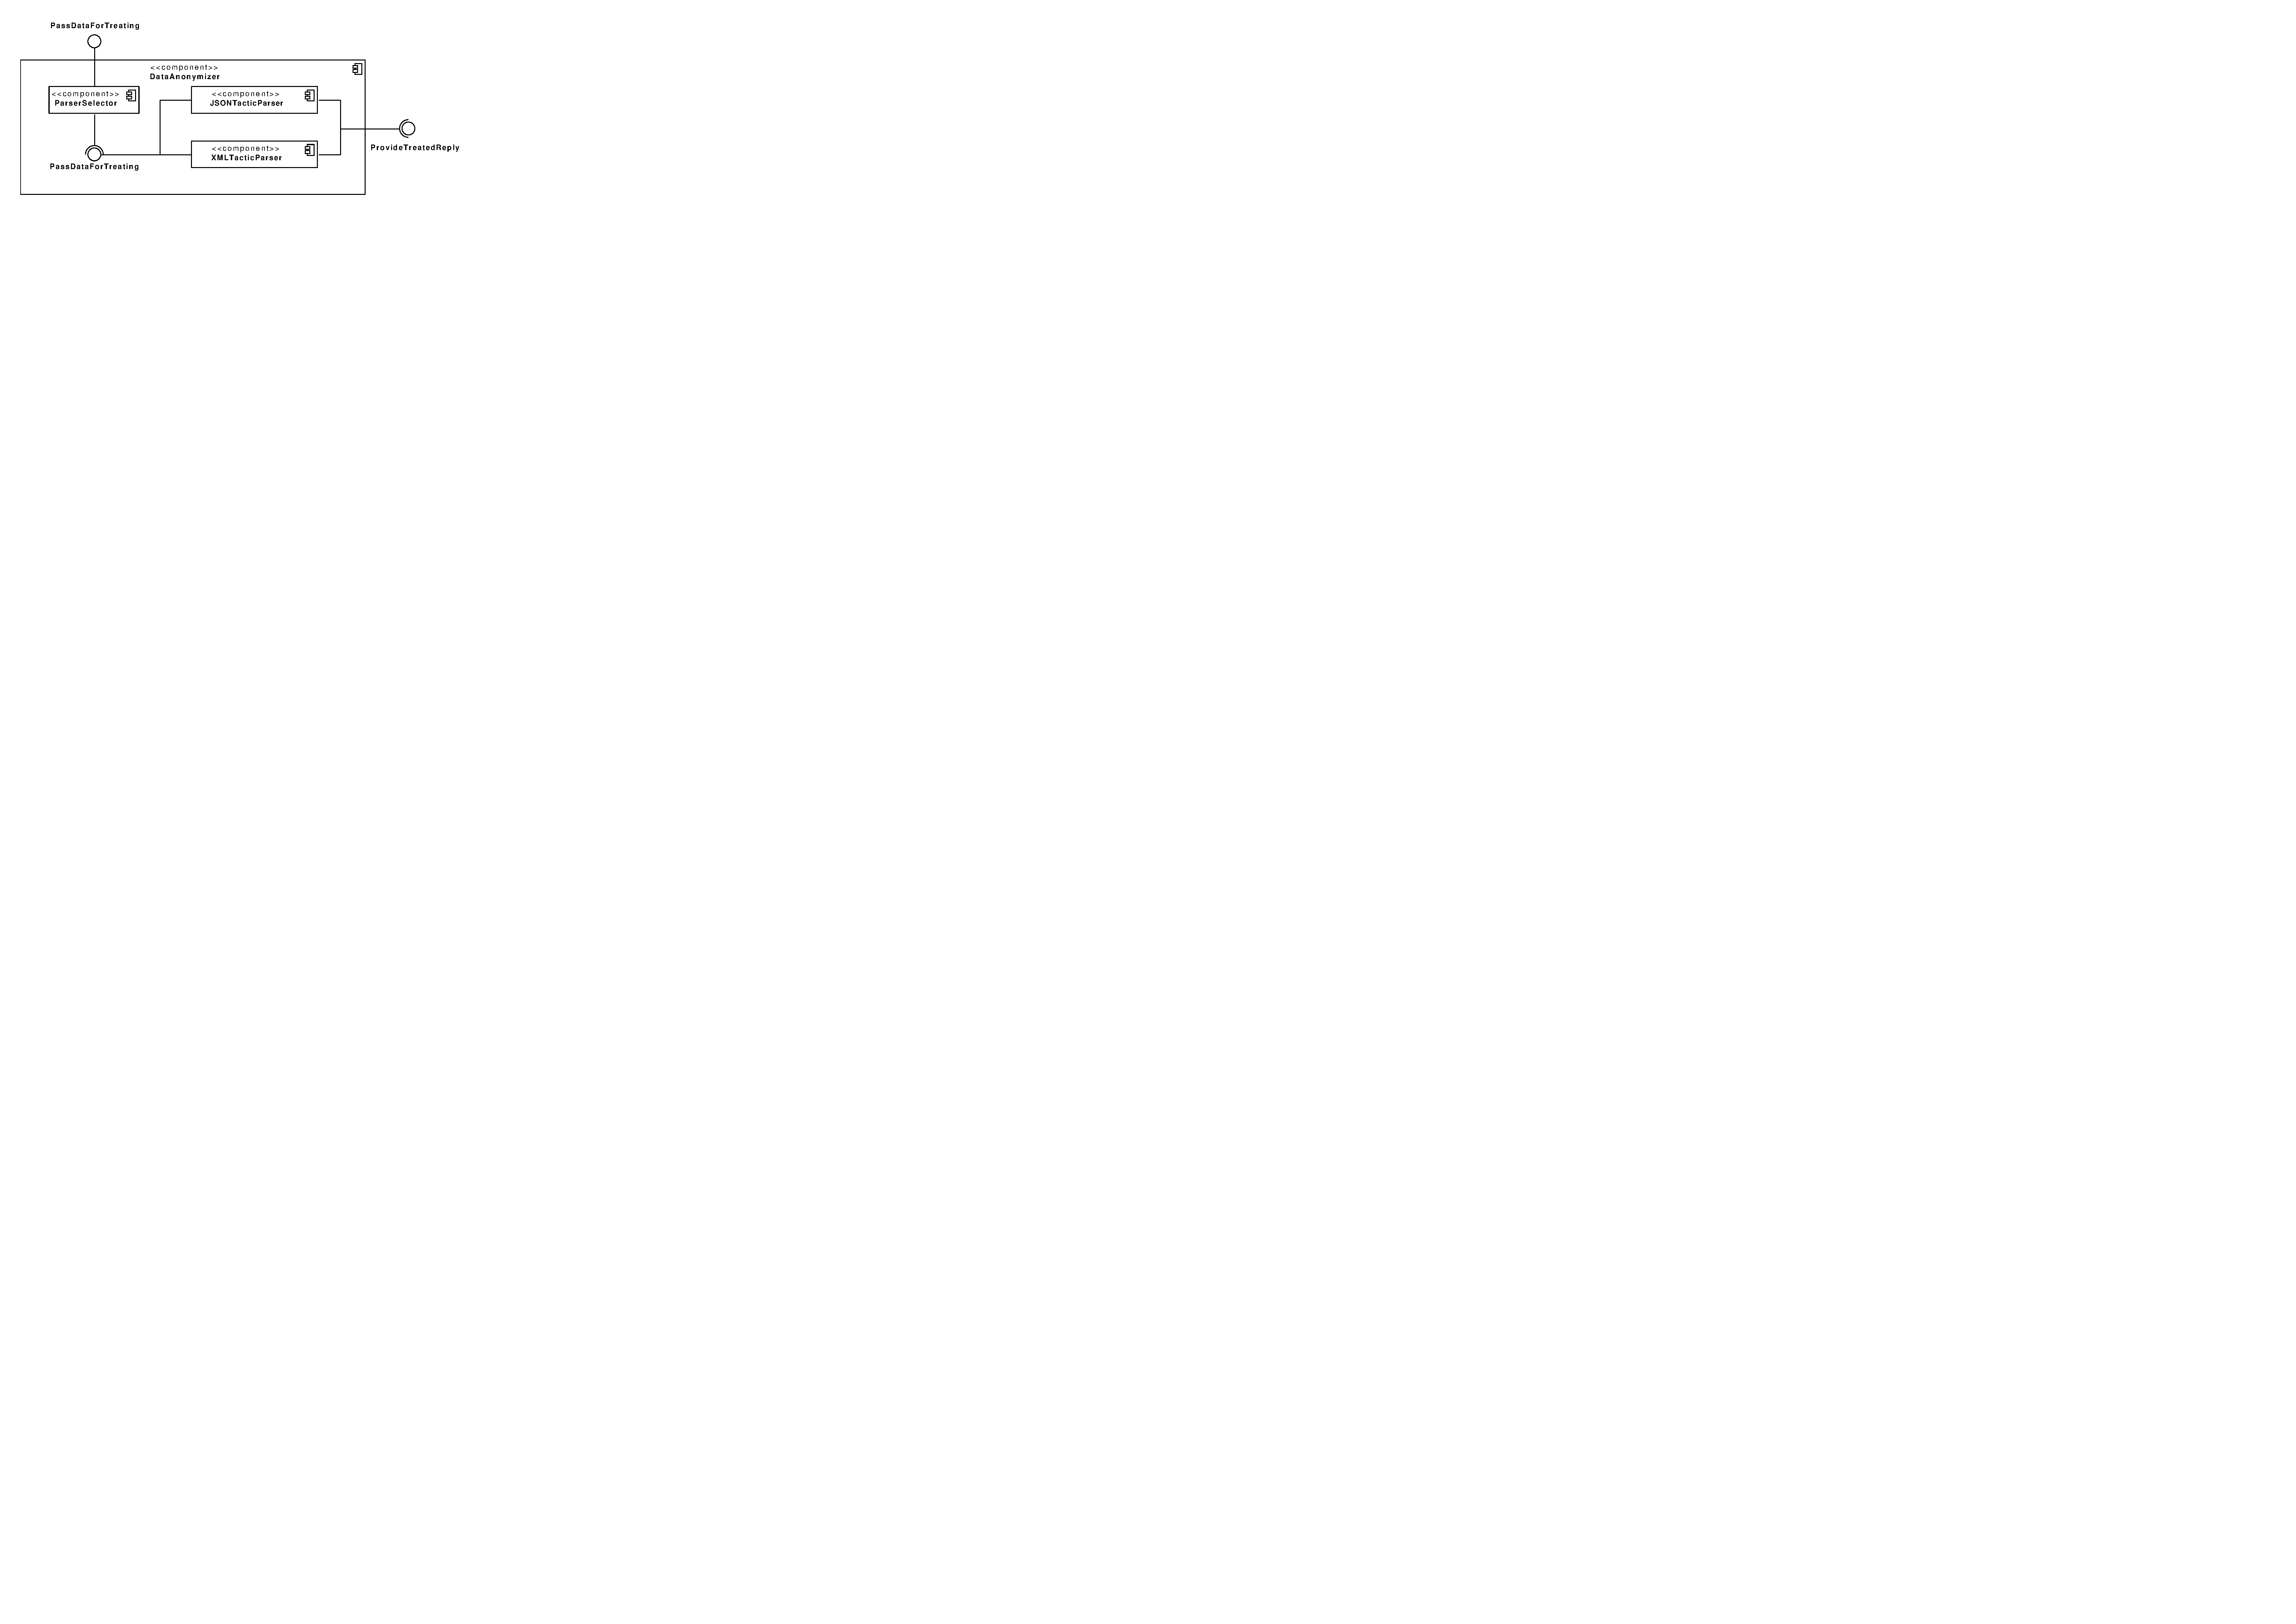
\includegraphics[width=\maxwidth{\textwidth}]{appendices/architecture/images/ComponentDiagram-DataAnonymizer-Component-Diagram.pdf}
  \caption[DataAnonymizer Component Diagram]{DataAnonymizer Component Diagram \label{diag:Component:DataAnonymizerComponentDiagram}}
\end{figure}

%%% DataTreatmentHandler Component Diagram (836.0x298.0)

\begin{figure}[!htp]
  \centering
  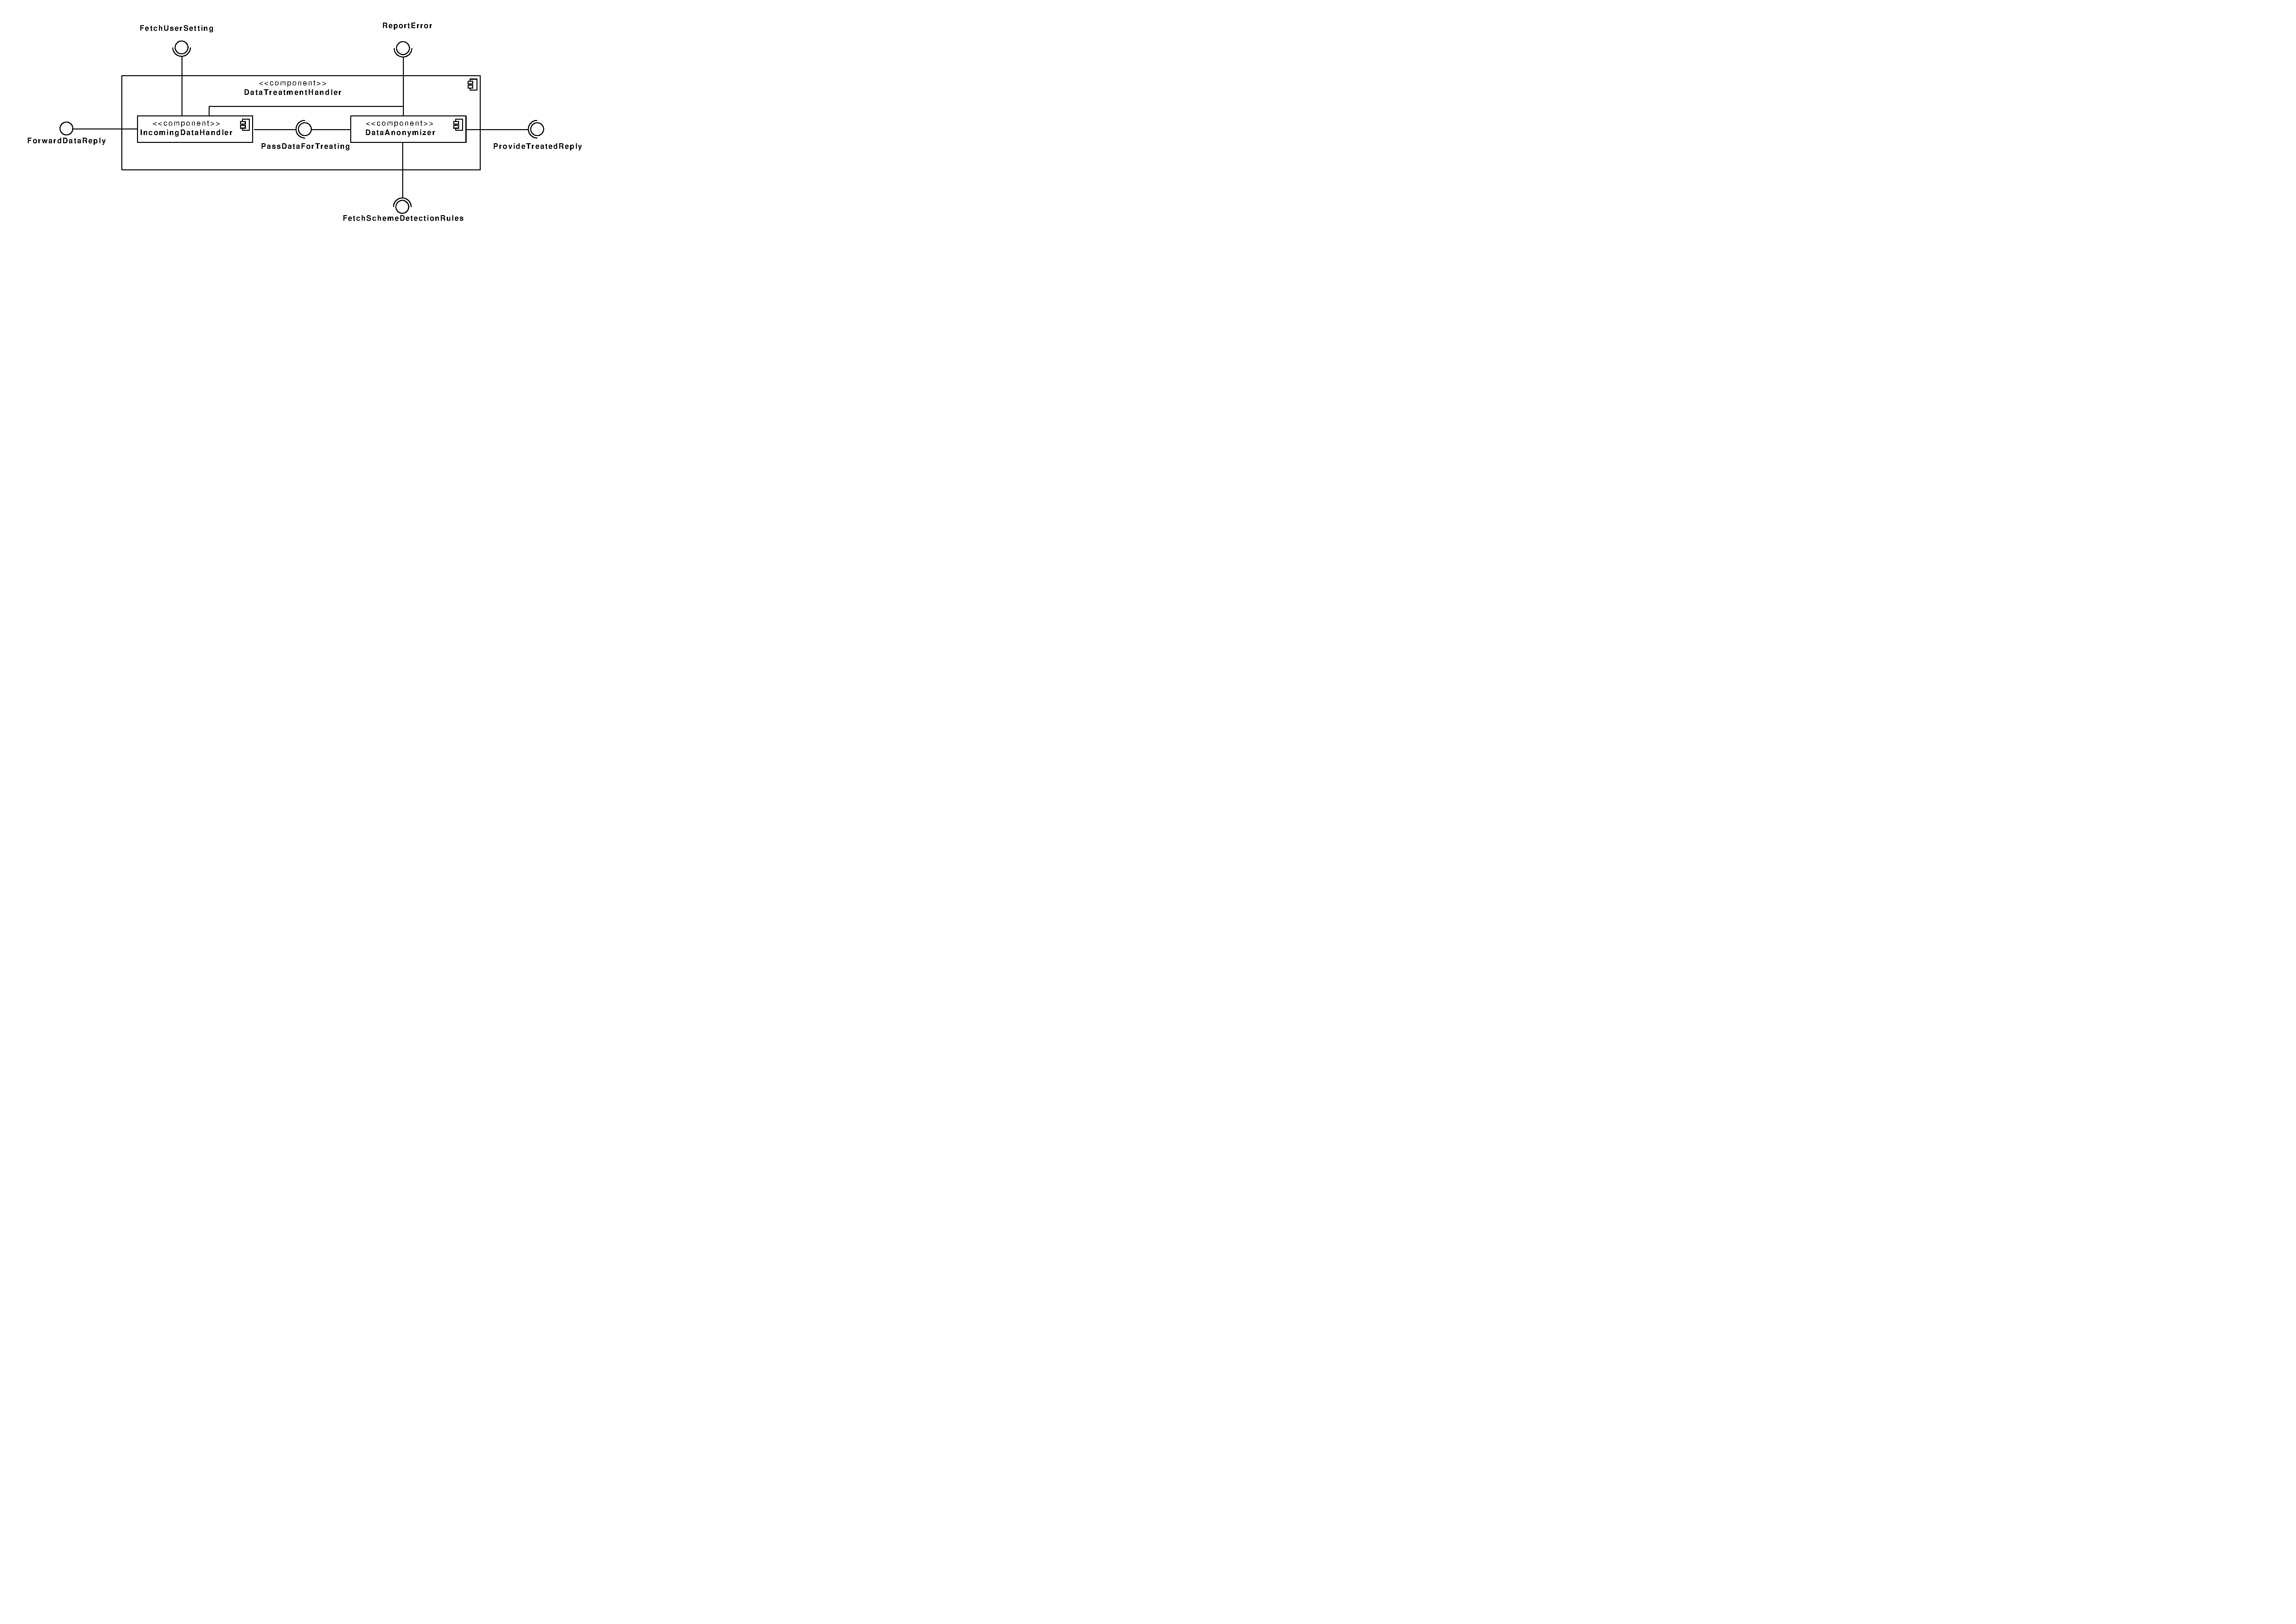
\includegraphics[width=\maxwidth{\textwidth}]{appendices/architecture/images/ComponentDiagram-DataTreatmentHandler-Component-Diagram.pdf}
  \caption[DataTreatmentHandler Component Diagram]{DataTreatmentHandler Component Diagram \label{diag:Component:DataTreatmentHandlerComponentDiagram}}
\end{figure}

%%% IncomingDataHandler Component Diagram (679.0x374.0)

\begin{figure}[!htp]
  \centering
  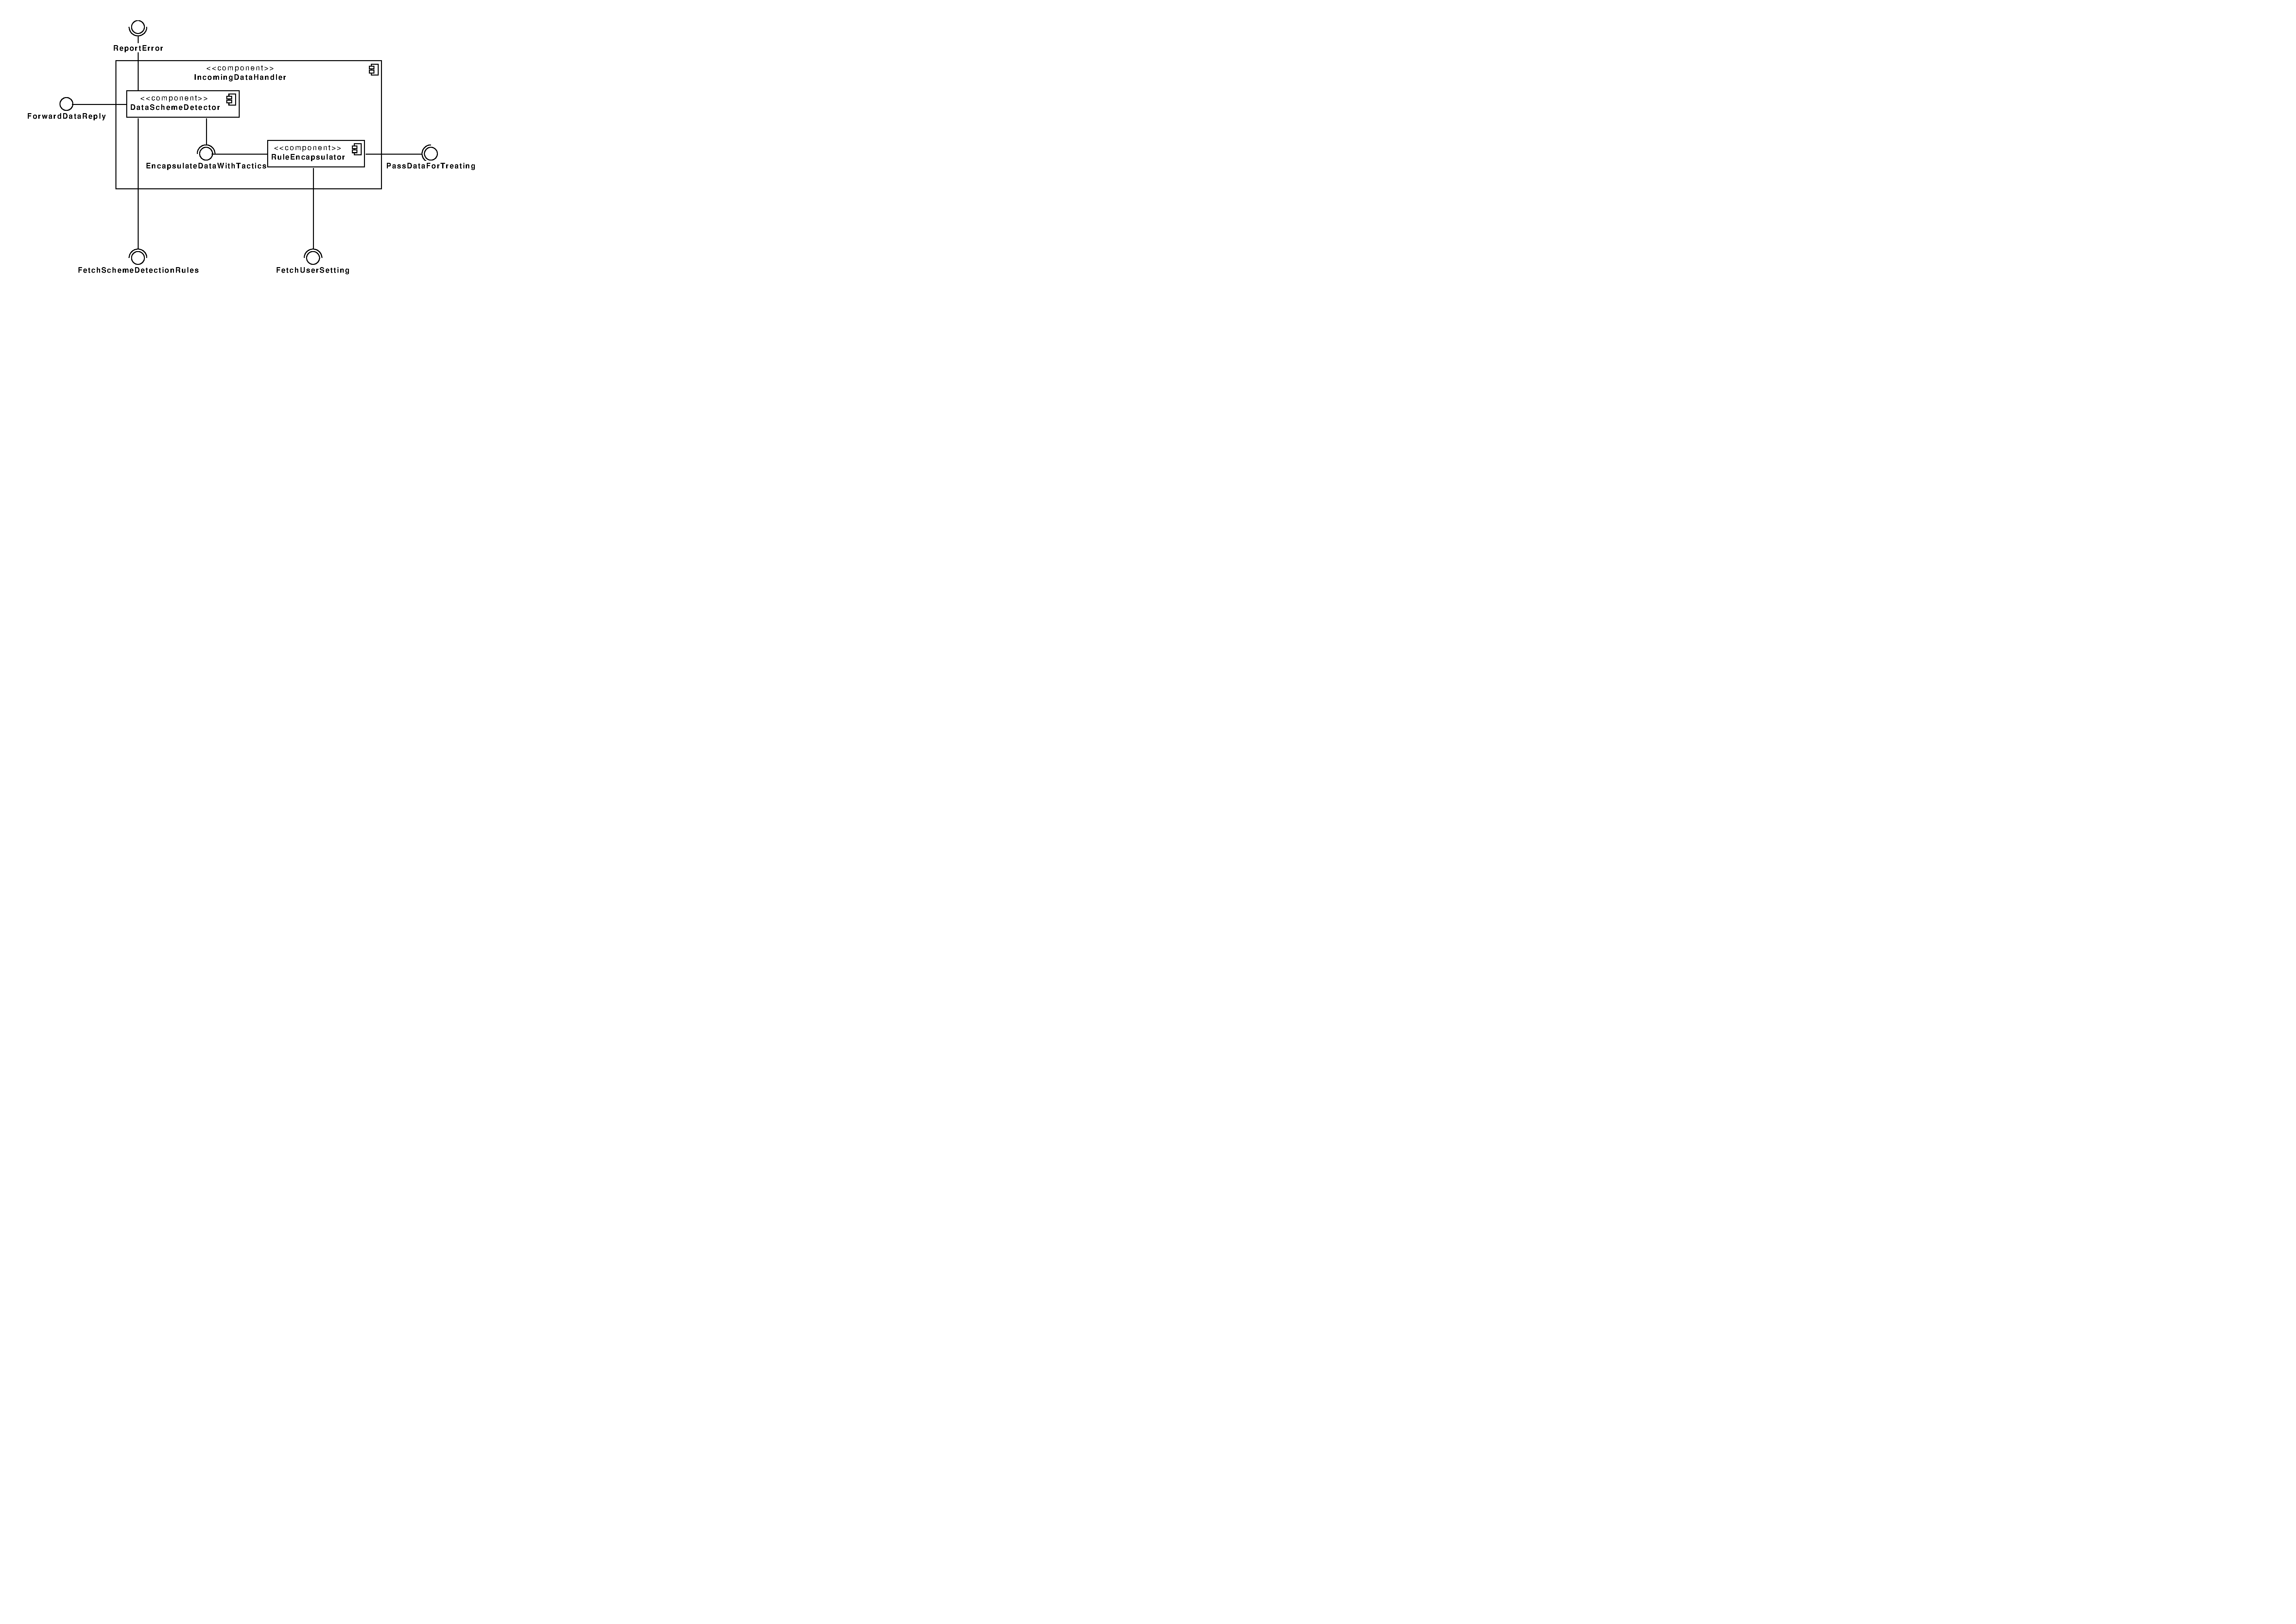
\includegraphics[width=\maxwidth{\textwidth}]{appendices/architecture/images/ComponentDiagram-IncomingDataHandler-Component-Diagram.pdf}
  \caption[IncomingDataHandler Component Diagram]{IncomingDataHandler Component Diagram \label{diag:Component:IncomingDataHandlerComponentDiagram}}
\end{figure}

%%% OutgoingHTTPHandler Component Diagram (833.0x316.0)

\begin{figure}[!htp]
  \centering
  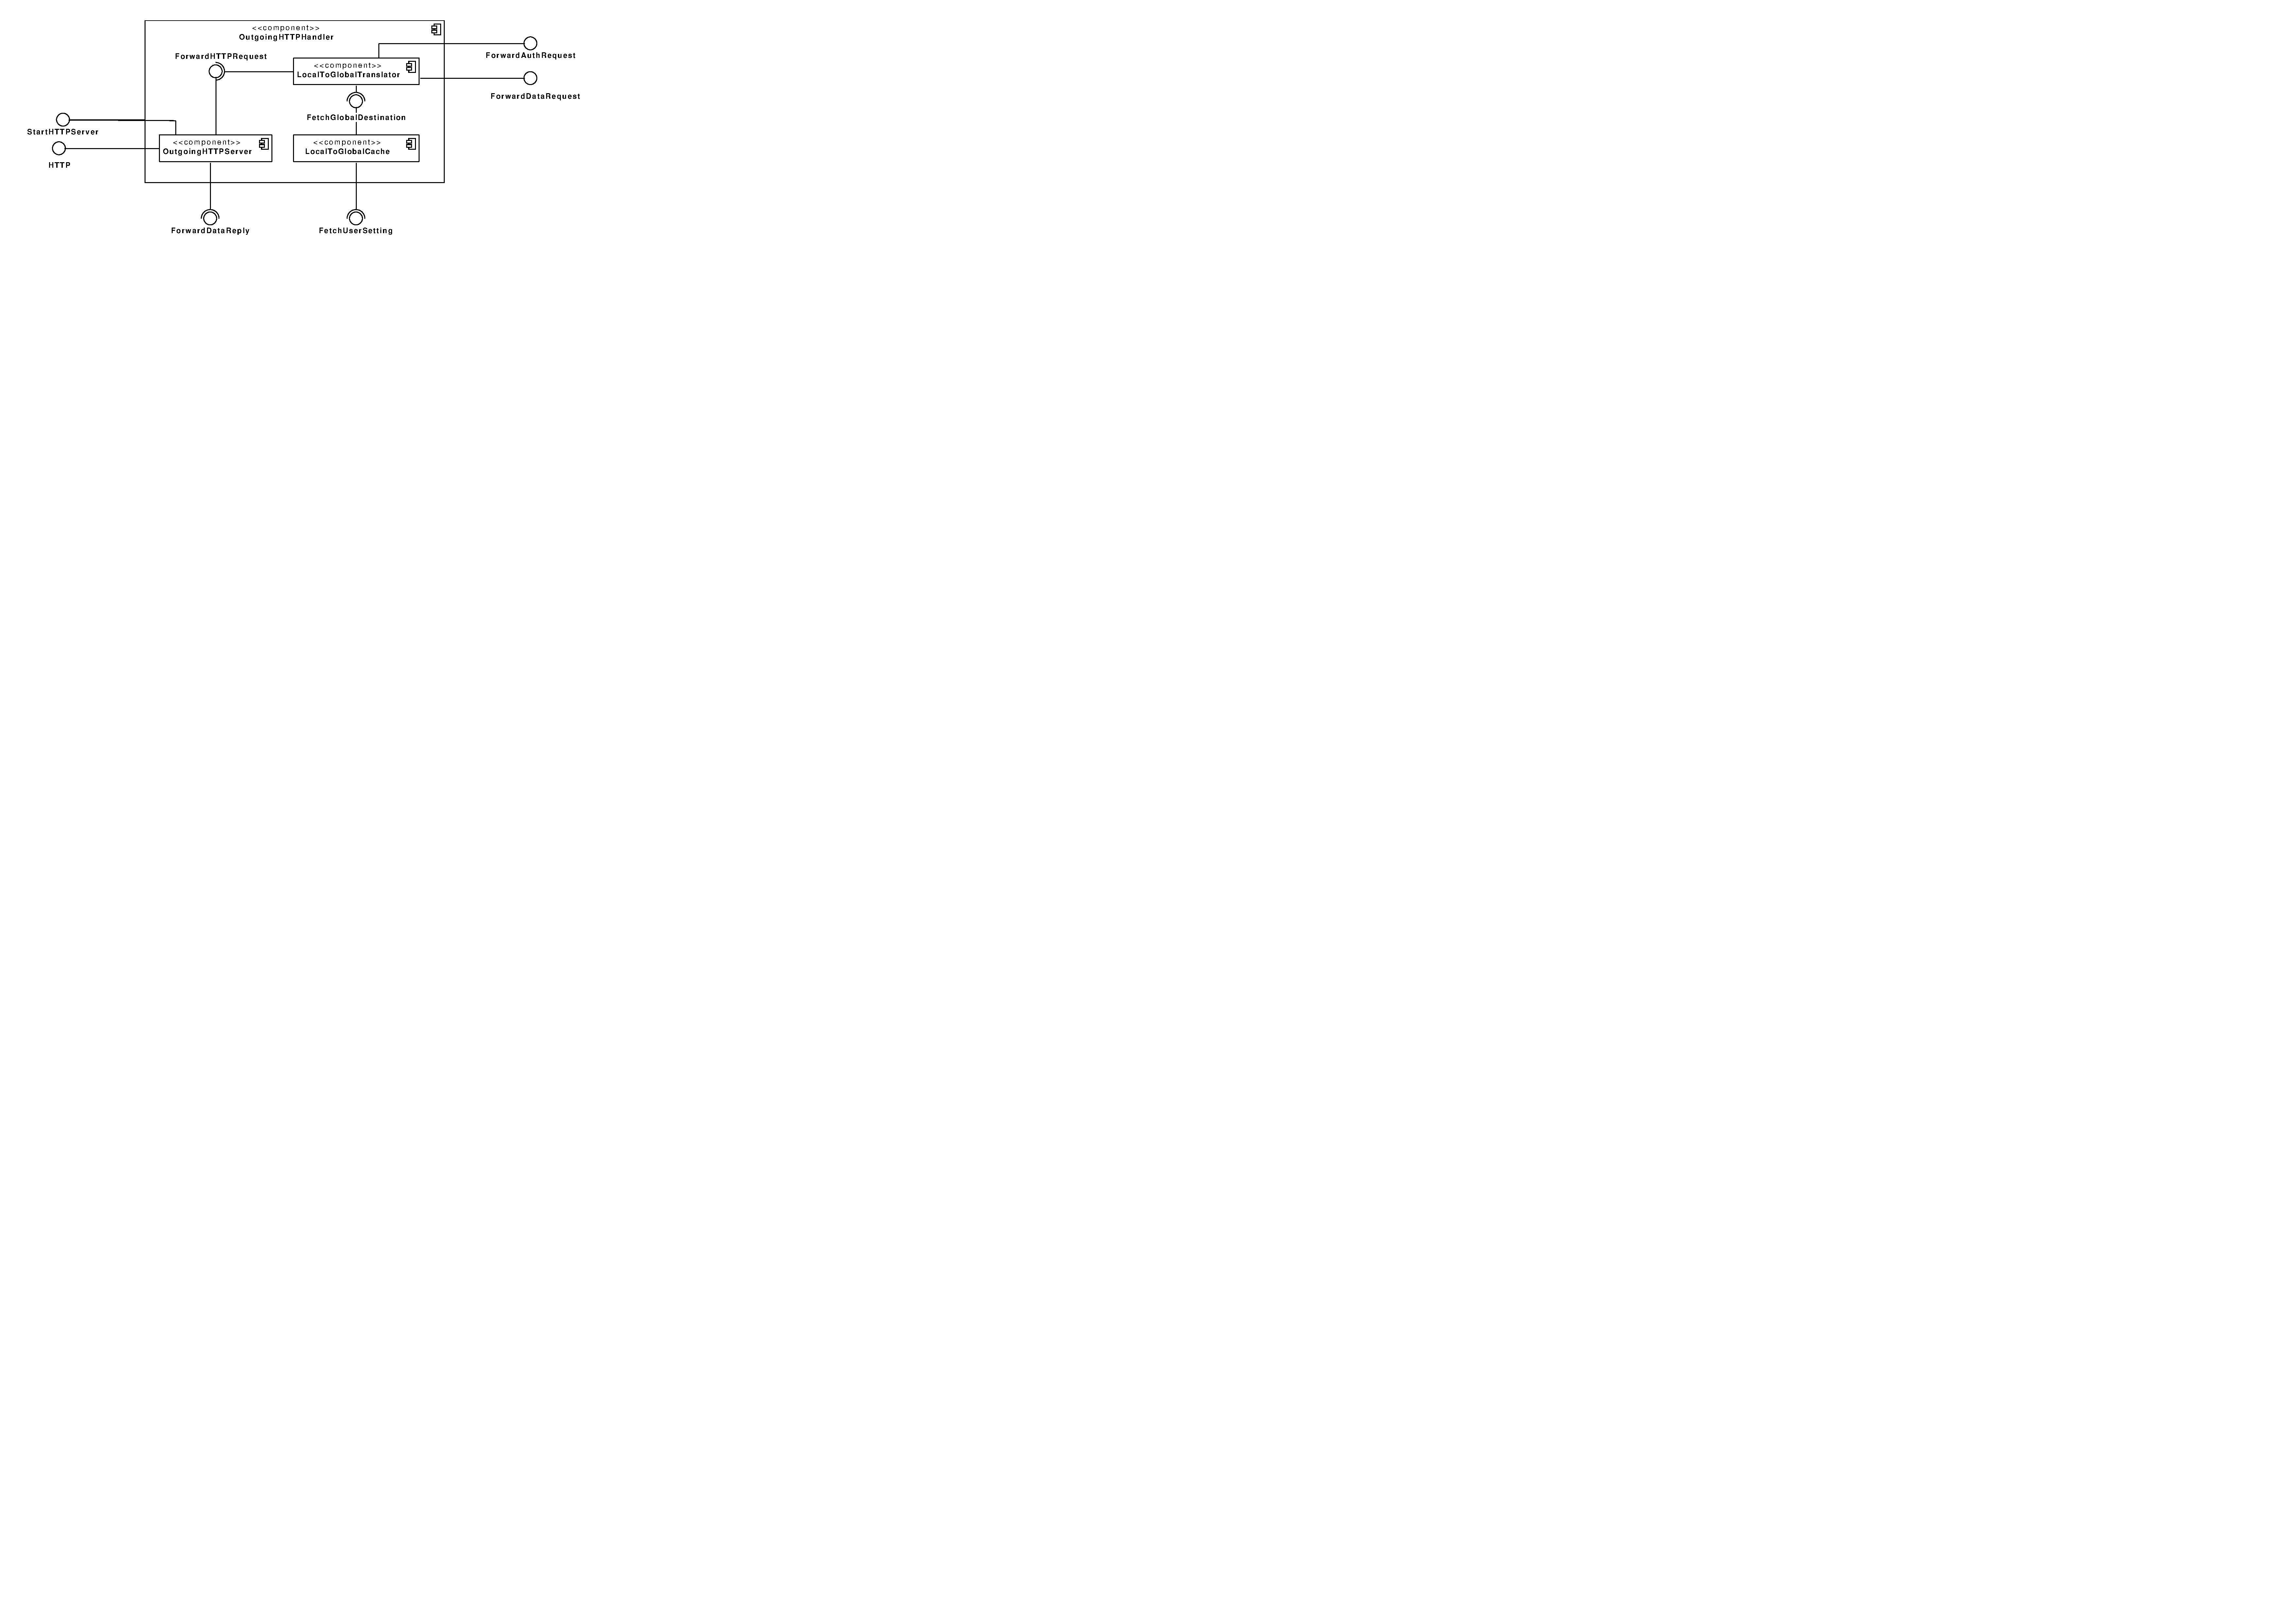
\includegraphics[width=\maxwidth{\textwidth}]{appendices/architecture/images/ComponentDiagram-OutgoingHTTPHandler-Component-Diagram.pdf}
  \caption[OutgoingHTTPHandler Component Diagram]{OutgoingHTTPHandler Component Diagram \label{diag:Component:OutgoingHTTPHandlerComponentDiagram}}
\end{figure}

%%% System Overview (927.0x393.0)

\begin{figure}[!htp]
  \centering
  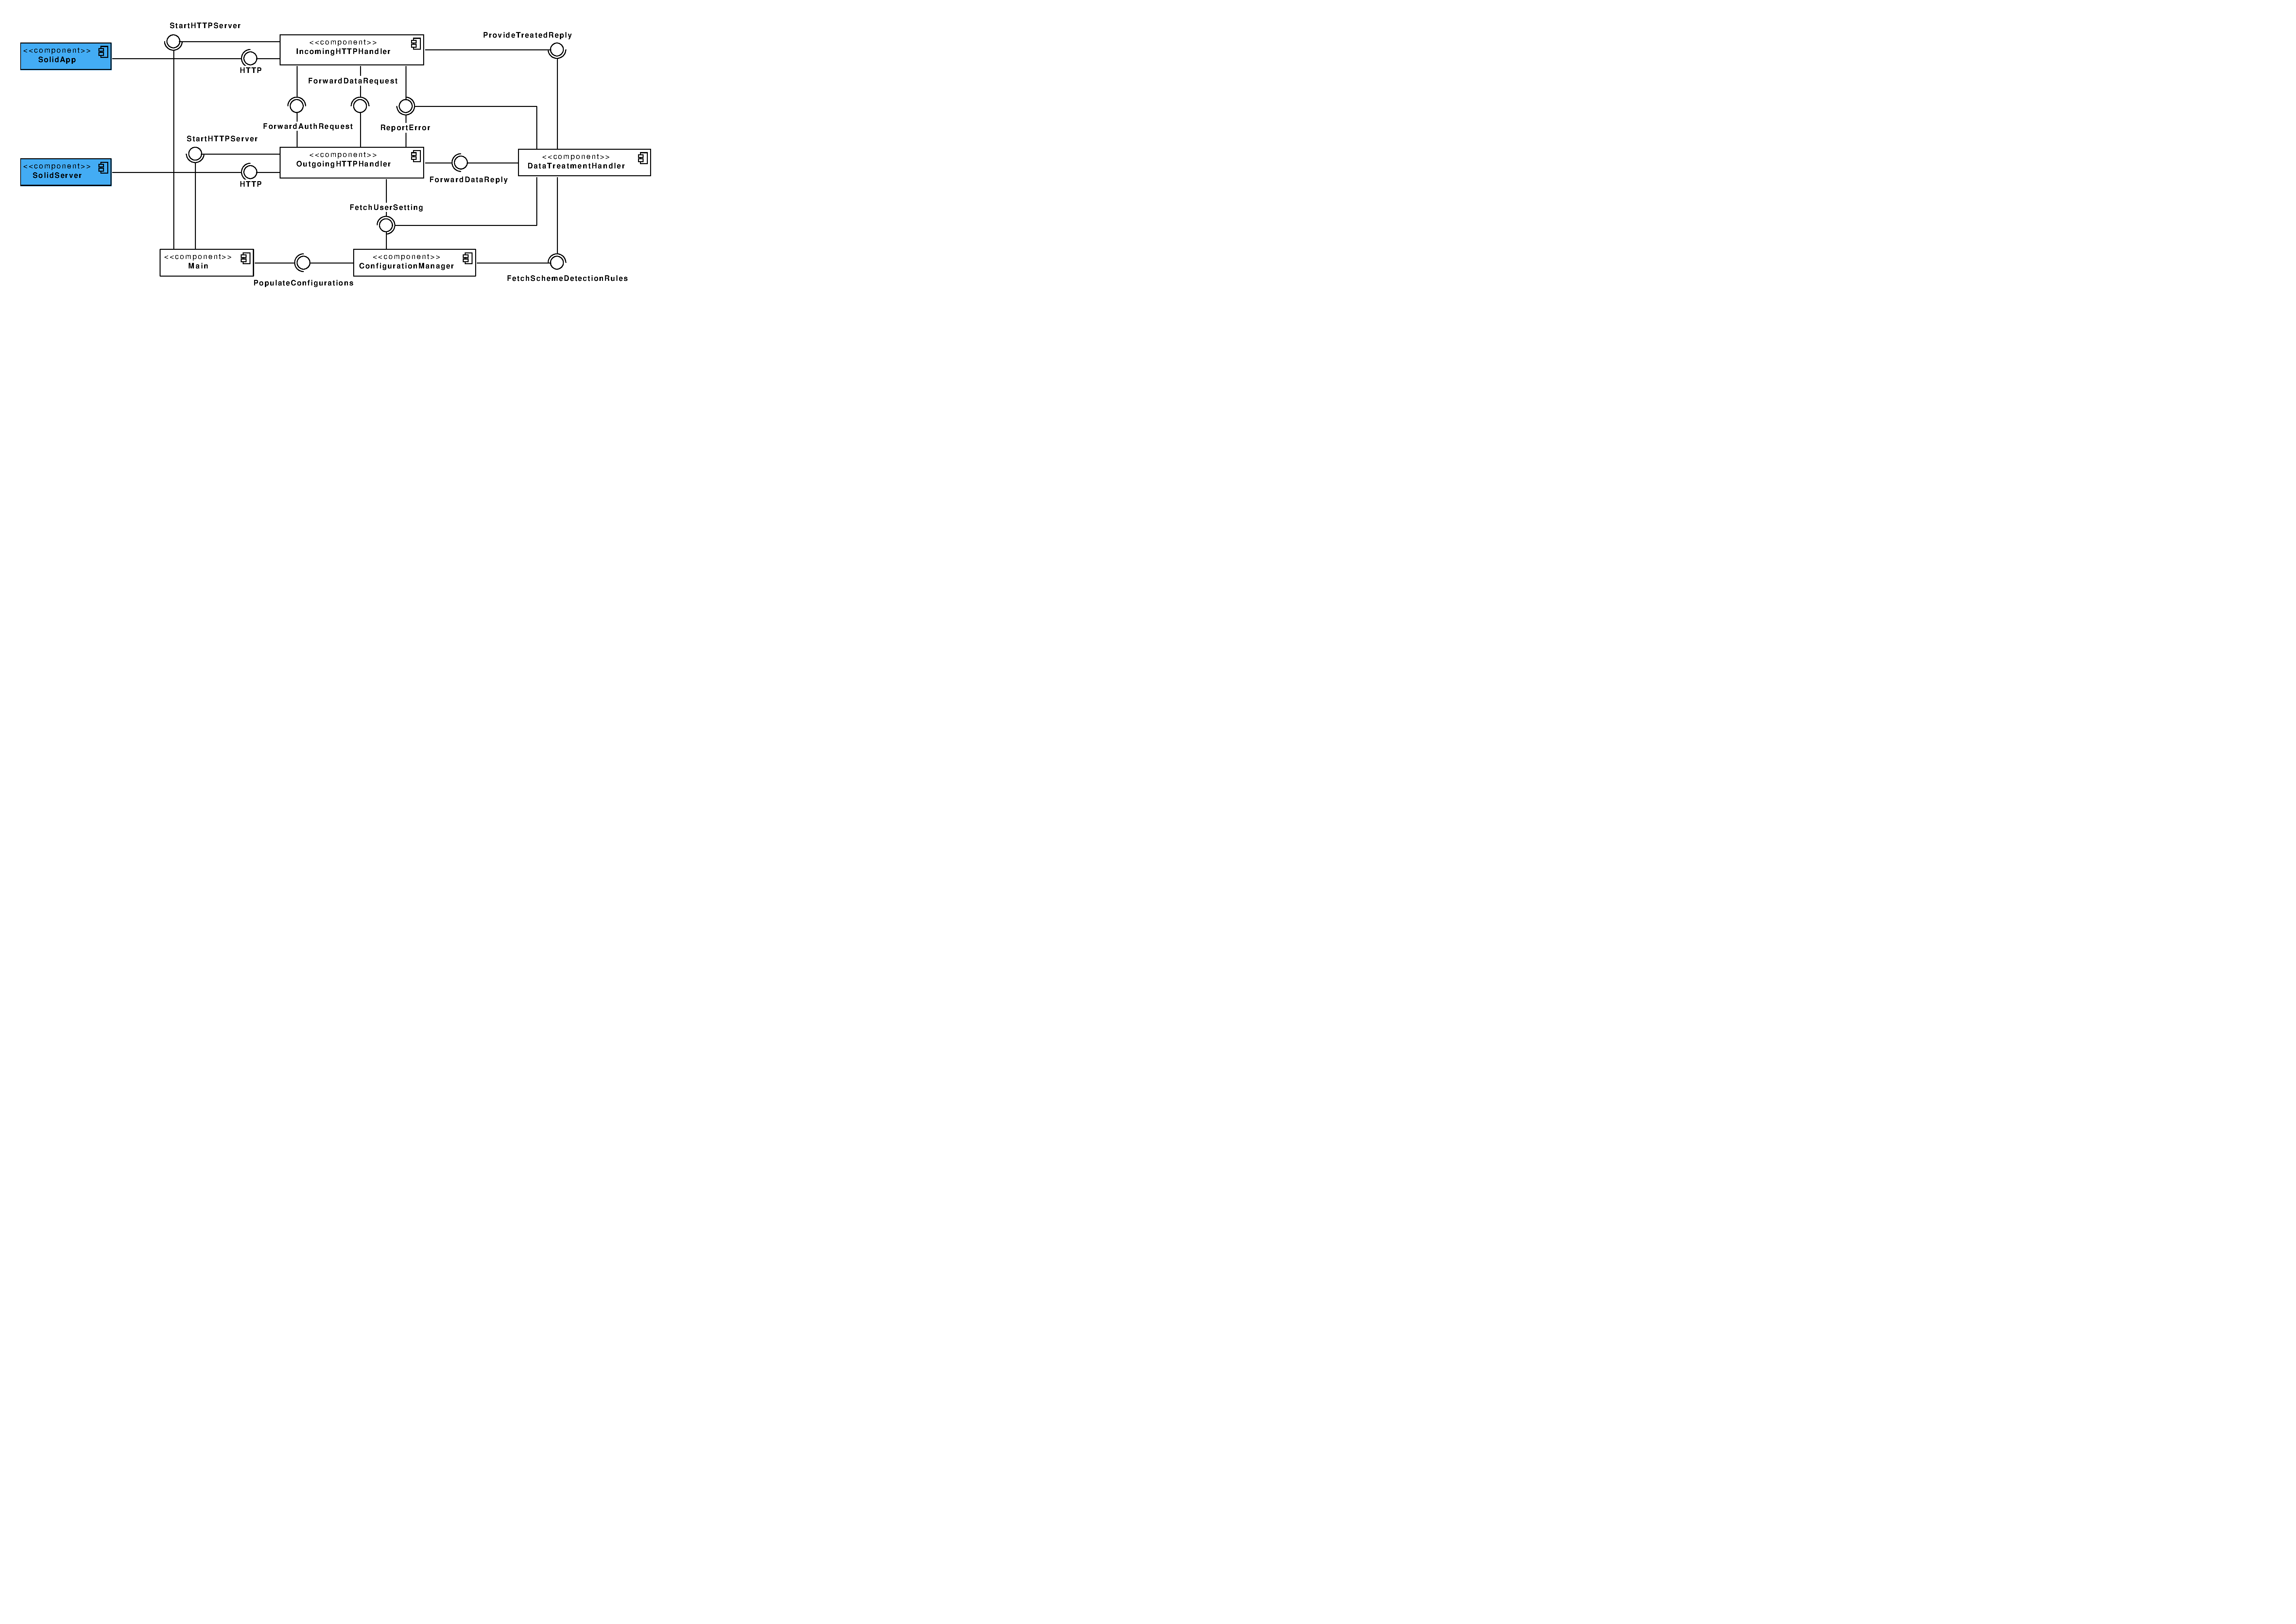
\includegraphics[width=\maxwidth{\textwidth}]{appendices/architecture/images/ComponentDiagram-System-Overview.pdf}
  \caption[System Overview]{System Overview \label{diag:Component:SystemOverview}}
\end{figure}



%%%%%%%%%%%%%%%%%%%%%%%%%%%%%%%%%%%%%%%%%%%%%%%%%%%%
%%% DEPLOYMENT
%%%%%%%%%%%%%%%%%%%%%%%%%%%%%%%%%%%%%%%%%%%%%%%%%%%%
\chapter{Deployment view (UML Deployment Diagram)}
\minilof{}




%%% Deployment Diagram (953.0x282.0)

\begin{figure}[!htp]
  \centering
  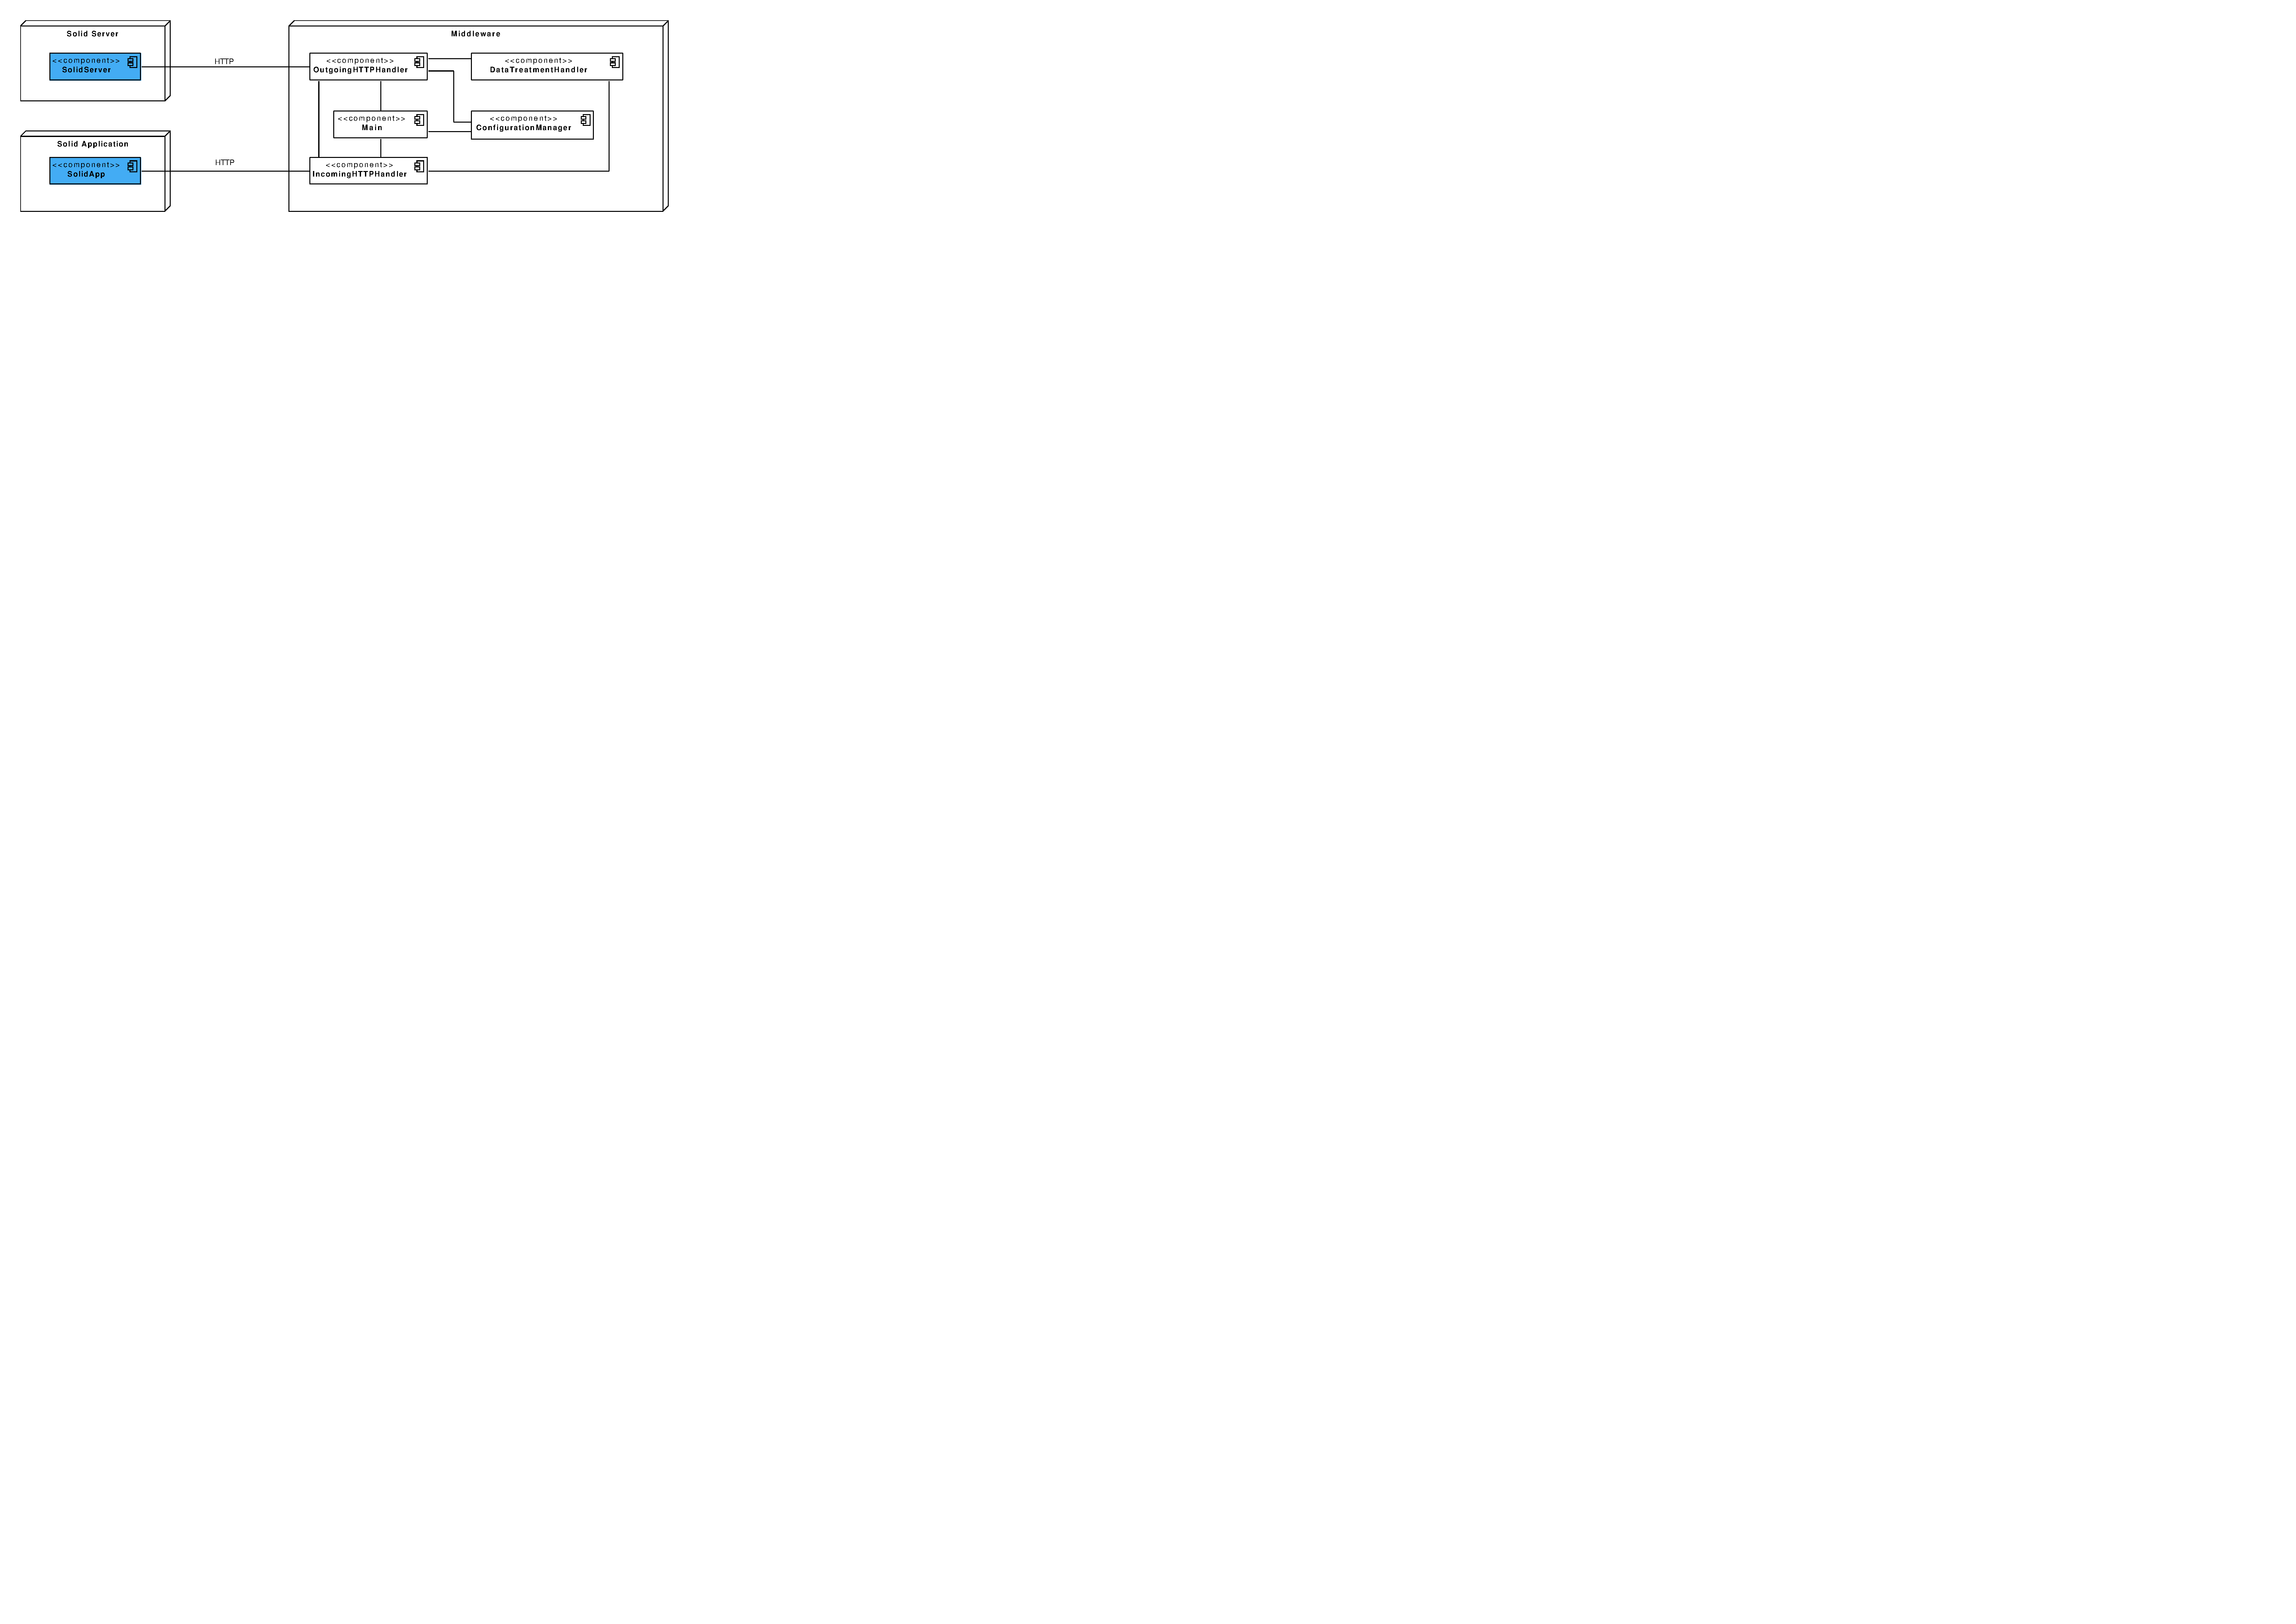
\includegraphics[width=\maxwidth{\textwidth}]{appendices/architecture/images/DeploymentDiagram-Deployment-Diagram.pdf}
  \caption[Deployment Diagram]{Deployment Diagram \label{diag:Deployment:DeploymentDiagram}}
\end{figure}



%%%%%%%%%%%%%%%%%%%%%%%%%%%%%%%%%%%%%%%%%%%%%%%%%%%%
%%% SEQUENCE
%%%%%%%%%%%%%%%%%%%%%%%%%%%%%%%%%%%%%%%%%%%%%%%%%%%%
\chapter{Process View (UML Sequence Diagram)}
\minilof{}


%%% Data flow (1305.0x406.0)

\begin{figure}[!htp]
  \centering
  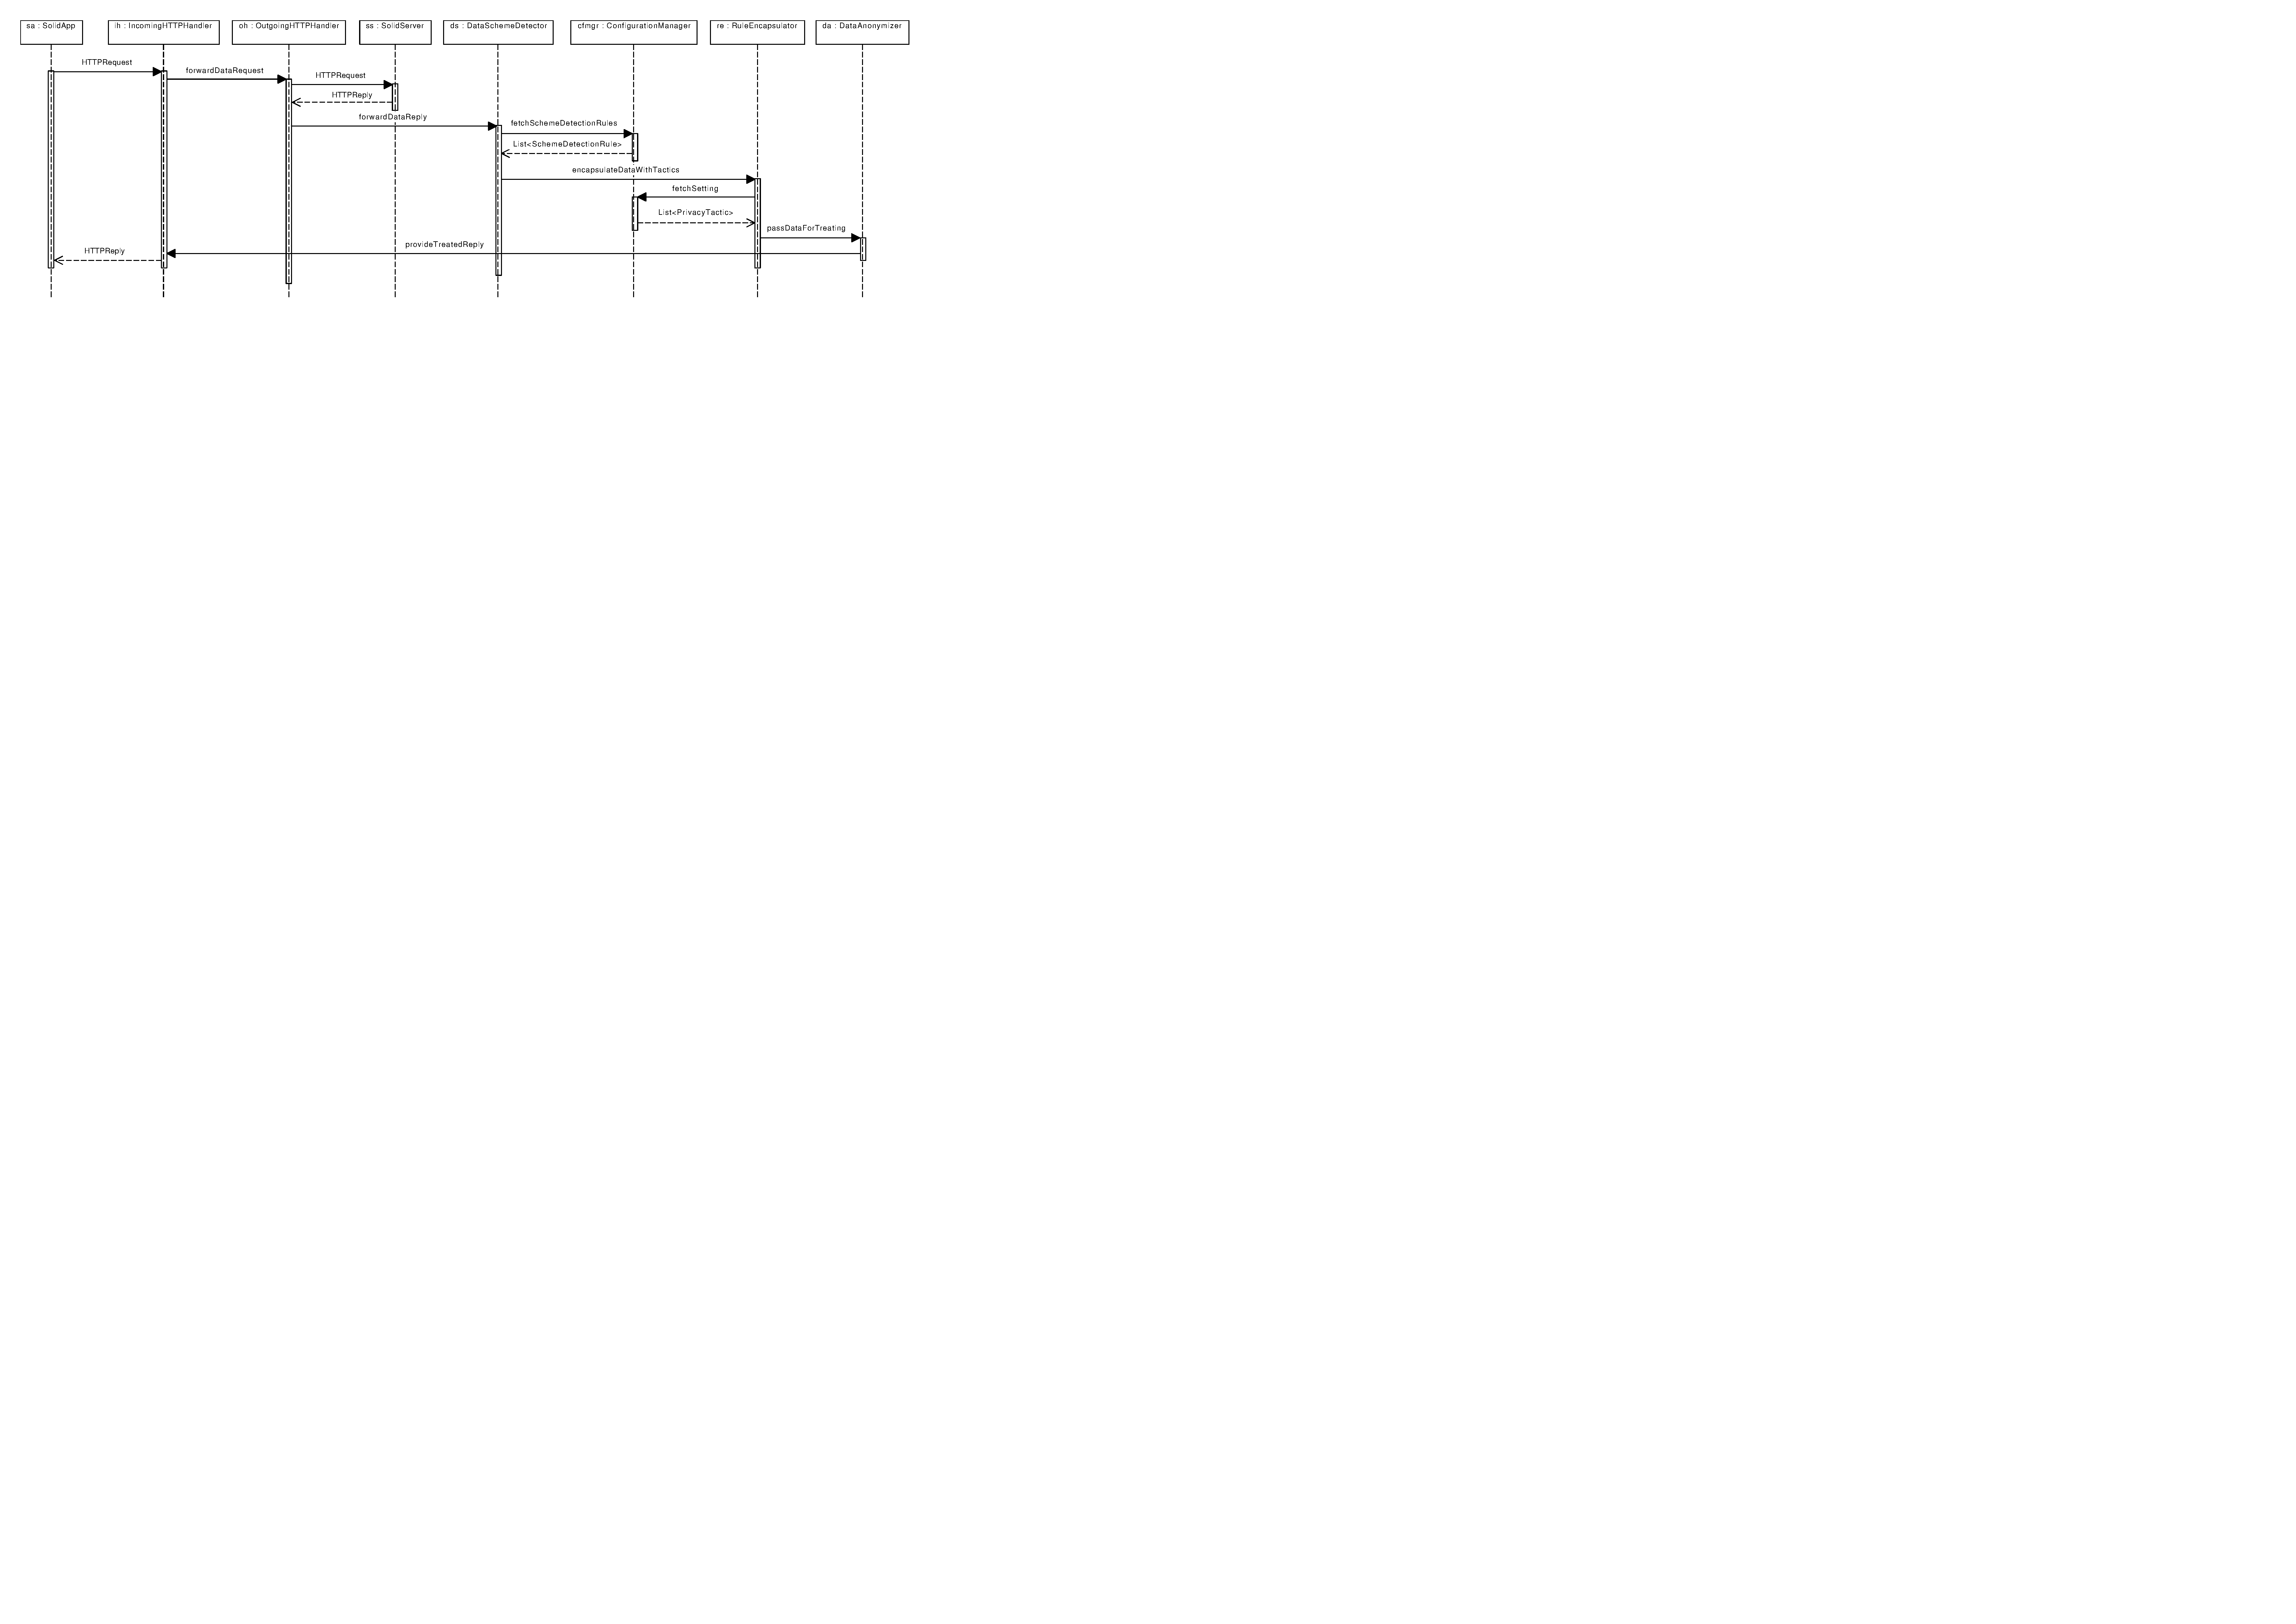
\includegraphics[width=\maxwidth{\textwidth}]{appendices/architecture/images/InteractionDiagram-Data-flow.pdf}
  \caption[Data flow]{Data flow \label{diag:Interaction:Dataflow}}
\end{figure}


% included tex file contains chapter command
%%% element catalog, generated on Sun Nov 28 22:49:53 CET 2021

%%% WARNING %%%
%%% This file was automatically generated by SAPlugin,
%%% and will be overwritten next time.

\chapter{Element catalog}\label{sec:catalog}
% COMPONENTS
\section{Components}\label{sec:components}
\subsection{ConfigurationManager}\label{comp:ComponentsConfigurationManager}
	\begin{description}[noitemsep,nolistsep]
		\item[Responsibility:]~The \vpett{\nameref{comp:ComponentsConfigurationManager}} component is responsible for storing all configurable settings, such as:
* The URL of the user's pod to connect to
* The URL the middleware should be deployed to
* A list of supported data schemes, and for each data scheme the settings as to which privacy level maps to which transformations
* Which privacy level should be applied (either by default, or for specific data schemes)
		\item[Super-components:]~None
		\item[Sub-components:]~None
		\item[Provided interfaces:]~\iconprovided{}~\vpett{\nameref{int:InterfacesFetchSchemeDetectionRules}}, \iconprovided{}~\vpett{\nameref{int:InterfacesFetchUserSetting}}, \iconprovided{}~\vpett{\nameref{int:InterfacesPopulateConfigurations}}
		\item[Required interfaces:]~None
		\item[Deployed on:]~\faSquareO~\vpett{\nameref{node:DeploymentMiddleware}}
		\item[Visible on diagrams:]~\cref{diag:Component:SystemOverview,diag:Deployment:DeploymentDiagram,diag:Interaction:Dataflow}		
	\end{description}

\subsection{DataAnonymizer}\label{comp:ComponentsDataTreatmentHandlerDataAnonymizer}
	\begin{description}[noitemsep,nolistsep]
		\item[Responsibility:]~The \vpett{\nameref{comp:ComponentsDataTreatmentHandlerDataAnonymizer}} is the main component responsible for taking in raw data (of which the scheme has already been detected, and the tactics necessary to be performed have been added to the data). It then performs all the required tactics on the data, using different components based on the content-representation of the data.
When no scheme is detected, a "\ref{data:ExceptionsNoMatchingSchemeException}" is thrown.
		\item[Super-components:]~\iconcomponent{}~\vpett{\nameref{comp:ComponentsDataTreatmentHandler}}
		\item[Sub-components:]~\iconcomponent{}~\vpett{\nameref{comp:ComponentsDataTreatmentHandlerDataAnonymizerJSONTacticParser}}, \iconcomponent{}~\vpett{\nameref{comp:ComponentsDataTreatmentHandlerDataAnonymizerXMLTacticParser}}, \iconcomponent{}~\vpett{\nameref{comp:ComponentsDataTreatmentHandlerDataAnonymizerParserSelector}}
		\item[Provided interfaces:]~\iconprovided{}~\vpett{\nameref{int:InterfacesPassDataForTreating}}
		\item[Required interfaces:]~\iconrequired{}~\vpett{\nameref{int:InterfacesFetchSchemeDetectionRules}}, \iconrequired{}~\vpett{\nameref{int:InterfacesProvideTreatedReply}}, \iconrequired{}~\vpett{\nameref{int:InterfacesReportError}}
		\item[Deployed on:]~\faSquareO~\vpett{\nameref{node:DeploymentMiddleware}}
		\item[Visible on diagrams:]~\cref{diag:Component:DataAnonymizerComponentDiagram,diag:Component:DataTreatmentHandlerComponentDiagram,diag:Interaction:Dataflow}		
	\end{description}

\subsection{DataSchemeDetector}\label{comp:ComponentsDataTreatmentHandlerIncomingDataHandlerDataSchemeDetector}
	\begin{description}[noitemsep,nolistsep]
		\item[Responsibility:]~The \vpett{\nameref{comp:ComponentsDataTreatmentHandlerIncomingDataHandlerDataSchemeDetector}} is the component responsible for taking in raw data, and then (using a set of SchemeDetectionRules), determining which scheme the data uses.
		\item[Super-components:]~\iconcomponent{}~\vpett{\nameref{comp:ComponentsDataTreatmentHandlerIncomingDataHandler}} $\triangleright$ \iconcomponent{}~\vpett{\nameref{comp:ComponentsDataTreatmentHandler}}
		\item[Sub-components:]~None
		\item[Provided interfaces:]~\iconprovided{}~\vpett{\nameref{int:InterfacesForwardDataReply}}, \iconprovided{}~\vpett{\nameref{int:InterfacesPassDataForTreating}}
		\item[Required interfaces:]~\iconrequired{}~\vpett{\nameref{int:InterfacesEncapsulateDataWithTactics}}, \iconrequired{}~\vpett{\nameref{int:InterfacesFetchSchemeDetectionRules}}, \iconrequired{}~\vpett{\nameref{int:InterfacesReportError}}
		\item[Deployed on:]~\faSquareO~\vpett{\nameref{node:DeploymentMiddleware}}
		\item[Visible on diagrams:]~\cref{diag:Component:IncomingDataHandlerComponentDiagram,diag:Interaction:Dataflow}		
	\end{description}

\subsection{DataTreatmentHandler}\label{comp:ComponentsDataTreatmentHandler}
	\begin{description}[noitemsep,nolistsep]
		\item[Responsibility:]~The DataRequestHandler forms the bulk of the application logic: it takes the replied data from the \vpett{\nameref{comp:ComponentsOutgoingHTTPHandler}}, and passes it through the \vpett{\nameref{comp:ComponentsDataTreatmentHandlerDataAnonymizer}} to apply the right transformations, before going through the OutgoingDataHandler to detect possible errors and return the transformed data to the \vpett{\nameref{comp:ComponentsIncomingHTTPHandler}}.
		\item[Super-components:]~None
		\item[Sub-components:]~\iconcomponent{}~\vpett{\nameref{comp:ComponentsDataTreatmentHandlerIncomingDataHandler}}, \iconcomponent{}~\vpett{\nameref{comp:ComponentsDataTreatmentHandlerDataAnonymizer}}
		\item[Provided interfaces:]~\iconprovided{}~\vpett{\nameref{int:InterfacesForwardDataReply}}
		\item[Required interfaces:]~\iconrequired{}~\vpett{\nameref{int:InterfacesFetchSchemeDetectionRules}}, \iconrequired{}~\vpett{\nameref{int:InterfacesFetchUserSetting}}, \iconrequired{}~\vpett{\nameref{int:InterfacesProvideTreatedReply}}, \iconrequired{}~\vpett{\nameref{int:InterfacesReportError}}
		\item[Deployed on:]~\faSquareO~\vpett{\nameref{node:DeploymentMiddleware}}
		\item[Visible on diagrams:]~\cref{diag:Component:DataTreatmentHandlerComponentDiagram,diag:Component:SystemOverview,diag:Deployment:DeploymentDiagram}		
	\end{description}

\subsection{IncomingDataHandler}\label{comp:ComponentsDataTreatmentHandlerIncomingDataHandler}
	\begin{description}[noitemsep,nolistsep]
		\item[Responsibility:]~The \vpett{\nameref{comp:ComponentsDataTreatmentHandlerIncomingDataHandler}} receives the data that is passed on from the \vpett{\nameref{comp:ComponentsOutgoingHTTPHandler}}. It then detects the scheme of the data and fetches the correct TransfromationRules to be applied to this data, which is then passed on to the \vpett{\nameref{comp:ComponentsDataTreatmentHandlerDataAnonymizer}}.
		\item[Super-components:]~\iconcomponent{}~\vpett{\nameref{comp:ComponentsDataTreatmentHandler}}
		\item[Sub-components:]~\iconcomponent{}~\vpett{\nameref{comp:ComponentsDataTreatmentHandlerIncomingDataHandlerRuleEncapsulator}}, \iconcomponent{}~\vpett{\nameref{comp:ComponentsDataTreatmentHandlerIncomingDataHandlerDataSchemeDetector}}
		\item[Provided interfaces:]~\iconprovided{}~\vpett{\nameref{int:InterfacesForwardDataReply}}
		\item[Required interfaces:]~\iconrequired{}~\vpett{\nameref{int:InterfacesFetchSchemeDetectionRules}}, \iconrequired{}~\vpett{\nameref{int:InterfacesFetchUserSetting}}, \iconrequired{}~\vpett{\nameref{int:InterfacesPassDataForTreating}}, \iconrequired{}~\vpett{\nameref{int:InterfacesReportError}}
		\item[Deployed on:]~\faSquareO~\vpett{\nameref{node:DeploymentMiddleware}}
		\item[Visible on diagrams:]~\cref{diag:Component:DataTreatmentHandlerComponentDiagram,diag:Component:IncomingDataHandlerComponentDiagram}		
	\end{description}

\subsection{IncomingHTTPHandler}\label{comp:ComponentsIncomingHTTPHandler}
	\begin{description}[noitemsep,nolistsep]
		\item[Responsibility:]~This component is responsible for handling incoming HTTP requests (i.e., from the Solid application, which sends a request to the solid server).
		\item[Super-components:]~None
		\item[Sub-components:]~None
		\item[Provided interfaces:]~\iconprovided{}~\vpett{\nameref{int:InterfacesHTTP}}, \iconprovided{}~\vpett{\nameref{int:InterfacesProvideTreatedReply}}, \iconprovided{}~\vpett{\nameref{int:InterfacesReportError}}, \iconprovided{}~\vpett{\nameref{int:InterfacesStartHTTPServer}}
		\item[Required interfaces:]~\iconrequired{}~\vpett{\nameref{int:InterfacesForwardAuthRequest}}, \iconrequired{}~\vpett{\nameref{int:InterfacesForwardDataRequest}}
		\item[Deployed on:]~\faSquareO~\vpett{\nameref{node:DeploymentMiddleware}}
		\item[Visible on diagrams:]~\cref{diag:Component:SystemOverview,diag:Deployment:DeploymentDiagram,diag:Interaction:Dataflow}		
	\end{description}

\subsection{JSONTacticParser}\label{comp:ComponentsDataTreatmentHandlerDataAnonymizerJSONTacticParser}
	\begin{description}[noitemsep,nolistsep]
		\item[Responsibility:]~The \vpett{\nameref{comp:ComponentsDataTreatmentHandlerDataAnonymizerJSONTacticParser}} is responsible for taking in the raw data (in JSON) and applying the encapsulated PrivacyTactics to the data before providing the treated data to the \vpett{\nameref{comp:ComponentsIncomingHTTPHandler}}.
		\item[Super-components:]~\iconcomponent{}~\vpett{\nameref{comp:ComponentsDataTreatmentHandlerDataAnonymizer}} $\triangleright$ \iconcomponent{}~\vpett{\nameref{comp:ComponentsDataTreatmentHandler}}
		\item[Sub-components:]~None
		\item[Provided interfaces:]~\iconprovided{}~\vpett{\nameref{int:InterfacesPassDataForTreating}}
		\item[Required interfaces:]~\iconrequired{}~\vpett{\nameref{int:InterfacesProvideTreatedReply}}
		\item[Deployed on:]~\faSquareO~\vpett{\nameref{node:DeploymentMiddleware}}
		\item[Visible on diagrams:]~\cref{diag:Component:DataAnonymizerComponentDiagram}		
	\end{description}

\subsection{LocalToGlobalCache}\label{comp:ComponentsOutgoingHTTPHandlerLocalToGlobalCache}
	\begin{description}[noitemsep,nolistsep]
		\item[Responsibility:]~The \vpett{\nameref{comp:ComponentsOutgoingHTTPHandlerLocalToGlobalCache}} is a cache that stores translations from the local to global destination. If no entry is found in the cache, the appropriate global destination is fetched from the \vpett{\nameref{comp:ComponentsConfigurationManager}}.
		\item[Super-components:]~\iconcomponent{}~\vpett{\nameref{comp:ComponentsOutgoingHTTPHandler}}
		\item[Sub-components:]~None
		\item[Provided interfaces:]~\iconprovided{}~\vpett{\nameref{int:InterfacesFetchGlobalDestination}}
		\item[Required interfaces:]~\iconrequired{}~\vpett{\nameref{int:InterfacesFetchUserSetting}}
		\item[Deployed on:]~\faSquareO~\vpett{\nameref{node:DeploymentMiddleware}}
		\item[Visible on diagrams:]~\cref{diag:Component:OutgoingHTTPHandlerComponentDiagram}		
	\end{description}

\subsection{LocalToGlobalTranslator}\label{comp:ComponentsOutgoingHTTPHandlerLocalToGlobalTranslator}
	\begin{description}[noitemsep,nolistsep]
		\item[Responsibility:]~The \vpett{\nameref{comp:ComponentsOutgoingHTTPHandlerLocalToGlobalTranslator}} is responsible for modifying an auth or data request, so that it can go to the \vpett{\nameref{comp:ComponentsOutgoingHTTPHandlerOutgoingHTTPServer}}. Concretely, when a request arrives, the URI still contains the domain of the middleware. This should be replaced with the domain of the \vpett{\nameref{comp:ComponentsSolidServer}}. The FetchGlobalDestination is used fetch the global destination.
		\item[Super-components:]~\iconcomponent{}~\vpett{\nameref{comp:ComponentsOutgoingHTTPHandler}}
		\item[Sub-components:]~None
		\item[Provided interfaces:]~\iconprovided{}~\vpett{\nameref{int:InterfacesForwardAuthRequest}}, \iconprovided{}~\vpett{\nameref{int:InterfacesForwardDataRequest}}
		\item[Required interfaces:]~\iconrequired{}~\vpett{\nameref{int:InterfacesFetchGlobalDestination}}, \iconrequired{}~\vpett{\nameref{int:InterfacesForwardHTTPRequest}}
		\item[Deployed on:]~\faSquareO~\vpett{\nameref{node:DeploymentMiddleware}}
		\item[Visible on diagrams:]~\cref{diag:Component:OutgoingHTTPHandlerComponentDiagram}		
	\end{description}

\subsection{Main}\label{comp:ComponentsMain}
	\begin{description}[noitemsep,nolistsep]
		\item[Responsibility:]~The entry-point of the program. This component is responsible for starting up the HTTP Server, and reading/parsing all configuration files (user settings and supported plugins/schemes).
		\item[Super-components:]~None
		\item[Sub-components:]~None
		\item[Provided interfaces:]~None
		\item[Required interfaces:]~\iconrequired{}~\vpett{\nameref{int:InterfacesPopulateConfigurations}}, \iconrequired{}~\vpett{\nameref{int:InterfacesStartHTTPServer}}
		\item[Deployed on:]~\faSquareO~\vpett{\nameref{node:DeploymentMiddleware}}
		\item[Visible on diagrams:]~\cref{diag:Component:SystemOverview,diag:Deployment:DeploymentDiagram}		
	\end{description}

\subsection{OutgoingHTTPHandler}\label{comp:ComponentsOutgoingHTTPHandler}
	\begin{description}[noitemsep,nolistsep]
		\item[Responsibility:]~The OutgoingHTTP is an HTTP client that is responsible for communication with the Solid server. When a data request is forwarded, it will send this request to the solid server, waiting for a reply, and then passing on the received data.
		\item[Super-components:]~None
		\item[Sub-components:]~\iconcomponent{}~\vpett{\nameref{comp:ComponentsOutgoingHTTPHandlerLocalToGlobalTranslator}}, \iconcomponent{}~\vpett{\nameref{comp:ComponentsOutgoingHTTPHandlerLocalToGlobalCache}}, \iconcomponent{}~\vpett{\nameref{comp:ComponentsOutgoingHTTPHandlerOutgoingHTTPServer}}
		\item[Provided interfaces:]~\iconprovided{}~\vpett{\nameref{int:InterfacesForwardAuthRequest}}, \iconprovided{}~\vpett{\nameref{int:InterfacesForwardDataRequest}}, \iconprovided{}~\vpett{\nameref{int:InterfacesHTTP}}, \iconprovided{}~\vpett{\nameref{int:InterfacesStartHTTPServer}}
		\item[Required interfaces:]~\iconrequired{}~\vpett{\nameref{int:InterfacesFetchUserSetting}}, \iconrequired{}~\vpett{\nameref{int:InterfacesForwardDataReply}}, \iconrequired{}~\vpett{\nameref{int:InterfacesReportError}}
		\item[Deployed on:]~\faSquareO~\vpett{\nameref{node:DeploymentMiddleware}}
		\item[Visible on diagrams:]~\cref{diag:Component:OutgoingHTTPHandlerComponentDiagram,diag:Component:SystemOverview,diag:Deployment:DeploymentDiagram,diag:Interaction:Dataflow}		
	\end{description}

\subsection{OutgoingHTTPServer}\label{comp:ComponentsOutgoingHTTPHandlerOutgoingHTTPServer}
	\begin{description}[noitemsep,nolistsep]
		\item[Responsibility:]~The \vpett{\nameref{comp:ComponentsOutgoingHTTPHandlerOutgoingHTTPServer}} is an HTTP Server responsible for communication with the \vpett{\nameref{comp:ComponentsSolidServer}}.
		\item[Super-components:]~\iconcomponent{}~\vpett{\nameref{comp:ComponentsOutgoingHTTPHandler}}
		\item[Sub-components:]~None
		\item[Provided interfaces:]~\iconprovided{}~\vpett{\nameref{int:InterfacesForwardHTTPRequest}}, \iconprovided{}~\vpett{\nameref{int:InterfacesHTTP}}, \iconprovided{}~\vpett{\nameref{int:InterfacesStartHTTPServer}}
		\item[Required interfaces:]~\iconrequired{}~\vpett{\nameref{int:InterfacesForwardDataReply}}
		\item[Deployed on:]~\faSquareO~\vpett{\nameref{node:DeploymentMiddleware}}
		\item[Visible on diagrams:]~\cref{diag:Component:OutgoingHTTPHandlerComponentDiagram}		
	\end{description}

\subsection{ParserSelector}\label{comp:ComponentsDataTreatmentHandlerDataAnonymizerParserSelector}
	\begin{description}[noitemsep,nolistsep]
		\item[Responsibility:]~The \vpett{\nameref{comp:ComponentsDataTreatmentHandlerDataAnonymizerParserSelector}} component is responsible for forwarding the data it receives to the correct TacticParser, based on the content-representation of the data.
		\item[Super-components:]~\iconcomponent{}~\vpett{\nameref{comp:ComponentsDataTreatmentHandlerDataAnonymizer}} $\triangleright$ \iconcomponent{}~\vpett{\nameref{comp:ComponentsDataTreatmentHandler}}
		\item[Sub-components:]~None
		\item[Provided interfaces:]~\iconprovided{}~\vpett{\nameref{int:InterfacesPassDataForTreating}}
		\item[Required interfaces:]~\iconrequired{}~\vpett{\nameref{int:InterfacesPassDataForTreating}}
		\item[Deployed on:]~\faSquareO~\vpett{\nameref{node:DeploymentMiddleware}}
		\item[Visible on diagrams:]~\cref{diag:Component:DataAnonymizerComponentDiagram}		
	\end{description}

\subsection{RuleEncapsulator}\label{comp:ComponentsDataTreatmentHandlerIncomingDataHandlerRuleEncapsulator}
	\begin{description}[noitemsep,nolistsep]
		\item[Responsibility:]~The \vpett{\nameref{comp:ComponentsDataTreatmentHandlerIncomingDataHandlerRuleEncapsulator}} is responsible for asking the \vpett{\nameref{comp:ComponentsConfigurationManager}} which privacy level corresponds to the given DataType. Then, it asks the \vpett{\nameref{comp:ComponentsConfigurationManager}} for a List of PrivacyTactics, which specify how the given data should be treated. Finally, an encapsulation datatype is constructed that contains all necessary information for the correct TacticParser to complete its work.
		\item[Super-components:]~\iconcomponent{}~\vpett{\nameref{comp:ComponentsDataTreatmentHandlerIncomingDataHandler}} $\triangleright$ \iconcomponent{}~\vpett{\nameref{comp:ComponentsDataTreatmentHandler}}
		\item[Sub-components:]~None
		\item[Provided interfaces:]~\iconprovided{}~\vpett{\nameref{int:InterfacesEncapsulateDataWithTactics}}
		\item[Required interfaces:]~\iconrequired{}~\vpett{\nameref{int:InterfacesFetchUserSetting}}, \iconrequired{}~\vpett{\nameref{int:InterfacesPassDataForTreating}}
		\item[Deployed on:]~\faSquareO~\vpett{\nameref{node:DeploymentMiddleware}}
		\item[Visible on diagrams:]~\cref{diag:Component:IncomingDataHandlerComponentDiagram,diag:Interaction:Dataflow}		
	\end{description}

\subsection{SolidApp}\label{comp:ComponentsSolidApp}
	\begin{description}[noitemsep,nolistsep]
		\item[Responsibility:]~This component represents the Solid Application the user wishes to connect to the middleware. It will send requests to the middleware, which will be forwarded to the Solid Server. When the server replies, the data is parsed, and a reply is sent to the application.
		\item[Super-components:]~None
		\item[Sub-components:]~None
		\item[Provided interfaces:]~None
		\item[Required interfaces:]~\iconrequired{}~\vpett{\nameref{int:InterfacesHTTP}}
		\item[Deployed on:]~\faSquareO~\vpett{\nameref{node:DeploymentSolidApplication}}
		\item[Visible on diagrams:]~\cref{diag:Component:SystemOverview,diag:Deployment:DeploymentDiagram,diag:Interaction:Dataflow}		
	\end{description}

\subsection{SolidServer}\label{comp:ComponentsSolidServer}
	\begin{description}[noitemsep,nolistsep]
		\item[Responsibility:]~This component represents the Solid server where the user's pod is stored. A reference to its URI is kept in the configuration file, which is loaded by the \vpett{\nameref{comp:ComponentsConfigurationManager}}. The middleware will connect to this server to fetch data, before processing it.
		\item[Super-components:]~None
		\item[Sub-components:]~None
		\item[Provided interfaces:]~None
		\item[Required interfaces:]~\iconrequired{}~\vpett{\nameref{int:InterfacesHTTP}}
		\item[Deployed on:]~\faSquareO~\vpett{\nameref{node:DeploymentSolidServer}}
		\item[Visible on diagrams:]~\cref{diag:Component:SystemOverview,diag:Deployment:DeploymentDiagram,diag:Interaction:Dataflow}		
	\end{description}

\subsection{XMLTacticParser}\label{comp:ComponentsDataTreatmentHandlerDataAnonymizerXMLTacticParser}
	\begin{description}[noitemsep,nolistsep]
		\item[Responsibility:]~The \vpett{\nameref{comp:ComponentsDataTreatmentHandlerDataAnonymizerXMLTacticParser}} is responsible for taking in the raw data (in XML) and applying the encapsulated PrivacyTactics to the data before providing the treated data to the \vpett{\nameref{comp:ComponentsIncomingHTTPHandler}}.
		\item[Super-components:]~\iconcomponent{}~\vpett{\nameref{comp:ComponentsDataTreatmentHandlerDataAnonymizer}} $\triangleright$ \iconcomponent{}~\vpett{\nameref{comp:ComponentsDataTreatmentHandler}}
		\item[Sub-components:]~None
		\item[Provided interfaces:]~\iconprovided{}~\vpett{\nameref{int:InterfacesPassDataForTreating}}
		\item[Required interfaces:]~\iconrequired{}~\vpett{\nameref{int:InterfacesProvideTreatedReply}}
		\item[Deployed on:]~\faSquareO~\vpett{\nameref{node:DeploymentMiddleware}}
		\item[Visible on diagrams:]~\cref{diag:Component:DataAnonymizerComponentDiagram}		
	\end{description}


% END COMPONENTS

% MODULES
% no modules
% END MODULES

% INTERFACES
\section{Interfaces} \label{sec:interfaces}
  %%%%%%%% EncapsulateDataWithTactics
  \subsection{EncapsulateDataWithTactics}\label{int:InterfacesEncapsulateDataWithTactics}
    \begin{description}[noitemsep,nolistsep]
      \item[Provided by:] \iconcomponent{}~\vpett{\nameref{comp:ComponentsDataTreatmentHandlerIncomingDataHandlerRuleEncapsulator}}
      \item[Required by:] \iconcomponent{}~\vpett{\nameref{comp:ComponentsDataTreatmentHandlerIncomingDataHandlerDataSchemeDetector}} 
           \item[Description]: This interface provides a method for the \vpett{\nameref{comp:ComponentsDataTreatmentHandlerIncomingDataHandlerDataSchemeDetector}} to pass its data, which now includes the detected DataScheme, to the \vpett{\nameref{comp:ComponentsDataTreatmentHandlerIncomingDataHandlerRuleEncapsulator}} which will encapsulate the PrivacyTactics that must be performed.
      \item[Operations:] ~
    \begin{itemize}[noitemsep,nolistsep,leftmargin=-.25cm]
      \item \textsf{void passToEncapsulate(\ref{data:DatatypesTreatableData} data, List\textless{}\ref{data:DatatypesPrivacyTactic}\textgreater{} tactics)}
        \begin{itemize}[noitemsep,nolistsep]
           \item Effect: This function takes the list of privacy tactics to be performed, and the data on which they should be performed, and passes it on to the \vpett{\nameref{comp:ComponentsDataTreatmentHandlerIncomingDataHandlerRuleEncapsulator}}. 
           \item Sequence Diagrams: None
        \end{itemize}
    \end{itemize}
      \item[Diagrams:] \cref{diag:Component:IncomingDataHandlerComponentDiagram}
    \end{description}

  %%%%%%%% FetchGlobalDestination
  \subsection{FetchGlobalDestination}\label{int:InterfacesFetchGlobalDestination}
    \begin{description}[noitemsep,nolistsep]
      \item[Provided by:] \iconcomponent{}~\vpett{\nameref{comp:ComponentsOutgoingHTTPHandlerLocalToGlobalCache}}
      \item[Required by:] \iconcomponent{}~\vpett{\nameref{comp:ComponentsOutgoingHTTPHandlerLocalToGlobalTranslator}} 
      \item[Operations:] ~
% no operations
      \item[Diagrams:] \cref{diag:Component:OutgoingHTTPHandlerComponentDiagram}
    \end{description}

  %%%%%%%% FetchSchemeDetectionRules
  \subsection{FetchSchemeDetectionRules}\label{int:InterfacesFetchSchemeDetectionRules}
    \begin{description}[noitemsep,nolistsep]
      \item[Provided by:] \iconcomponent{}~\vpett{\nameref{comp:ComponentsConfigurationManager}}
      \item[Required by:] \iconcomponent{}~\vpett{\nameref{comp:ComponentsDataTreatmentHandlerDataAnonymizer}}, \iconcomponent{}~\vpett{\nameref{comp:ComponentsDataTreatmentHandlerIncomingDataHandlerDataSchemeDetector}}, \iconcomponent{}~\vpett{\nameref{comp:ComponentsDataTreatmentHandler}}, \iconcomponent{}~\vpett{\nameref{comp:ComponentsDataTreatmentHandlerIncomingDataHandler}} 
           \item[Description]: This interface provides a method to retrieve a List<\ref{data:DatatypesSchemeDetectionRule}>, which are used to identify the resulting data scheme.
      \item[Operations:] ~
    \begin{itemize}[noitemsep,nolistsep,leftmargin=-.25cm]
      \item \textsf{List\textless{}\ref{data:DatatypesSchemeDetectionRule}\textgreater{} fetchSchemeDetectionRules()}
        \begin{itemize}[noitemsep,nolistsep]
           \item Effect: {\colorbox{red!30}{\underline{Undefined}}} 
           \item Returns: A list of SchemeDetectionRules to find the correct data scheme.
           \item Sequence Diagrams: None
        \end{itemize}
    \end{itemize}
      \item[Diagrams:] \cref{diag:Component:DataTreatmentHandlerComponentDiagram,diag:Component:IncomingDataHandlerComponentDiagram,diag:Component:SystemOverview}
    \end{description}

  %%%%%%%% FetchUserSetting
  \subsection{FetchUserSetting}\label{int:InterfacesFetchUserSetting}
    \begin{description}[noitemsep,nolistsep]
      \item[Provided by:] \iconcomponent{}~\vpett{\nameref{comp:ComponentsConfigurationManager}}
      \item[Required by:] \iconcomponent{}~\vpett{\nameref{comp:ComponentsDataTreatmentHandler}}, \iconcomponent{}~\vpett{\nameref{comp:ComponentsDataTreatmentHandlerIncomingDataHandler}}, \iconcomponent{}~\vpett{\nameref{comp:ComponentsOutgoingHTTPHandlerLocalToGlobalCache}}, \iconcomponent{}~\vpett{\nameref{comp:ComponentsOutgoingHTTPHandler}}, \iconcomponent{}~\vpett{\nameref{comp:ComponentsDataTreatmentHandlerIncomingDataHandlerRuleEncapsulator}} 
           \item[Description]: This interface is responsible for providing information configured by the user. Examples include fetching the user's pod URI, the URL the server should run on and the settings pertaining to the requested privacy levels.
      \item[Operations:] ~
    \begin{itemize}[noitemsep,nolistsep,leftmargin=-.25cm]
      \item \textsf{string fetchSetting(string setting)}
        \begin{itemize}[noitemsep,nolistsep]
           \item Effect: {\colorbox{red!30}{\underline{Undefined}}} 
           \item Returns: The requested UserSetting
           \item Sequence Diagrams: None
        \end{itemize}
    \end{itemize}
      \item[Diagrams:] \cref{diag:Component:DataTreatmentHandlerComponentDiagram,diag:Component:IncomingDataHandlerComponentDiagram,diag:Component:OutgoingHTTPHandlerComponentDiagram,diag:Component:SystemOverview}
    \end{description}

  %%%%%%%% ForwardAuthRequest
  \subsection{ForwardAuthRequest}\label{int:InterfacesForwardAuthRequest}
    \begin{description}[noitemsep,nolistsep]
      \item[Provided by:] \iconcomponent{}~\vpett{\nameref{comp:ComponentsOutgoingHTTPHandlerLocalToGlobalTranslator}}, \iconcomponent{}~\vpett{\nameref{comp:ComponentsOutgoingHTTPHandler}}
      \item[Required by:] \iconcomponent{}~\vpett{\nameref{comp:ComponentsIncomingHTTPHandler}} 
           \item[Description]: Forward an authentication request to the \vpett{\nameref{comp:ComponentsOutgoingHTTPHandler}}, to make sure authentication is handled by the \vpett{\nameref{comp:ComponentsSolidServer}}.
      \item[Operations:] ~
    \begin{itemize}[noitemsep,nolistsep,leftmargin=-.25cm]
      \item \textsf{void forwardRequest(string data)}
        \begin{itemize}[noitemsep,nolistsep]
           \item Effect: {\colorbox{red!30}{\underline{Undefined}}} 
           \item Sequence Diagrams: None
        \end{itemize}
    \end{itemize}
      \item[Diagrams:] \cref{diag:Component:OutgoingHTTPHandlerComponentDiagram,diag:Component:SystemOverview}
    \end{description}

  %%%%%%%% ForwardDataReply
  \subsection{ForwardDataReply}\label{int:InterfacesForwardDataReply}
    \begin{description}[noitemsep,nolistsep]
      \item[Provided by:] \iconcomponent{}~\vpett{\nameref{comp:ComponentsDataTreatmentHandlerIncomingDataHandlerDataSchemeDetector}}, \iconcomponent{}~\vpett{\nameref{comp:ComponentsDataTreatmentHandler}}, \iconcomponent{}~\vpett{\nameref{comp:ComponentsDataTreatmentHandlerIncomingDataHandler}}
      \item[Required by:] \iconcomponent{}~\vpett{\nameref{comp:ComponentsOutgoingHTTPHandler}}, \iconcomponent{}~\vpett{\nameref{comp:ComponentsOutgoingHTTPHandlerOutgoingHTTPServer}} 
      \item[Operations:] ~
    \begin{itemize}[noitemsep,nolistsep,leftmargin=-.25cm]
      \item \textsf{void forwardDataReply(\ref{data:DatatypesDataReply} data)}
        \begin{itemize}[noitemsep,nolistsep]
           \item Effect: This operation forwards the data that the \vpett{\nameref{comp:ComponentsOutgoingHTTPHandlerOutgoingHTTPServer}} receives from the \vpett{\nameref{comp:ComponentsSolidServer}} to the DataRequestHandler, to be processed accordingly. 
           \item Sequence Diagrams: None
        \end{itemize}
    \end{itemize}
      \item[Diagrams:] \cref{diag:Component:DataTreatmentHandlerComponentDiagram,diag:Component:IncomingDataHandlerComponentDiagram,diag:Component:OutgoingHTTPHandlerComponentDiagram,diag:Component:SystemOverview}
    \end{description}

  %%%%%%%% ForwardDataRequest
  \subsection{ForwardDataRequest}\label{int:InterfacesForwardDataRequest}
    \begin{description}[noitemsep,nolistsep]
      \item[Provided by:] \iconcomponent{}~\vpett{\nameref{comp:ComponentsOutgoingHTTPHandlerLocalToGlobalTranslator}}, \iconcomponent{}~\vpett{\nameref{comp:ComponentsOutgoingHTTPHandler}}
      \item[Required by:] \iconcomponent{}~\vpett{\nameref{comp:ComponentsIncomingHTTPHandler}} 
      \item[Operations:] ~
    \begin{itemize}[noitemsep,nolistsep,leftmargin=-.25cm]
      \item \textsf{void forwardDataRequest(string data)}
        \begin{itemize}[noitemsep,nolistsep]
           \item Effect: Forward the data request to the \vpett{\nameref{comp:ComponentsOutgoingHTTPHandler}} 
           \item Sequence Diagrams: None
        \end{itemize}
    \end{itemize}
      \item[Diagrams:] \cref{diag:Component:OutgoingHTTPHandlerComponentDiagram,diag:Component:SystemOverview}
    \end{description}

  %%%%%%%% ForwardHTTPRequest
  \subsection{ForwardHTTPRequest}\label{int:InterfacesForwardHTTPRequest}
    \begin{description}[noitemsep,nolistsep]
      \item[Provided by:] \iconcomponent{}~\vpett{\nameref{comp:ComponentsOutgoingHTTPHandlerOutgoingHTTPServer}}
      \item[Required by:] \iconcomponent{}~\vpett{\nameref{comp:ComponentsOutgoingHTTPHandlerLocalToGlobalTranslator}} 
           \item[Description]: This interface provides a method to forward an HTTPRequest from the \vpett{\nameref{comp:ComponentsOutgoingHTTPHandlerLocalToGlobalTranslator}} to the \vpett{\nameref{comp:ComponentsOutgoingHTTPHandlerOutgoingHTTPServer}}.
      \item[Operations:] ~
    \begin{itemize}[noitemsep,nolistsep,leftmargin=-.25cm]
      \item \textsf{void forwardHTTPRequest(\ref{data:DatatypesDataRequest} httpData)}
        \begin{itemize}[noitemsep,nolistsep]
           \item Effect: {\colorbox{red!30}{\underline{Undefined}}} 
           \item Sequence Diagrams: None
        \end{itemize}
    \end{itemize}
      \item[Diagrams:] \cref{diag:Component:OutgoingHTTPHandlerComponentDiagram}
    \end{description}

  %%%%%%%% HTTP
  \subsection{HTTP}\label{int:InterfacesHTTP}
    \begin{description}[noitemsep,nolistsep]
      \item[Provided by:] \iconcomponent{}~\vpett{\nameref{comp:ComponentsIncomingHTTPHandler}}, \iconcomponent{}~\vpett{\nameref{comp:ComponentsOutgoingHTTPHandler}}, \iconcomponent{}~\vpett{\nameref{comp:ComponentsOutgoingHTTPHandlerOutgoingHTTPServer}}
      \item[Required by:] \iconcomponent{}~\vpett{\nameref{comp:ComponentsSolidApp}}, \iconcomponent{}~\vpett{\nameref{comp:ComponentsSolidServer}} 
      \item[Operations:] ~
    \begin{itemize}[noitemsep,nolistsep,leftmargin=-.25cm]
      \item \textsf{void HTTPReply()}
        \begin{itemize}[noitemsep,nolistsep]
           \item Effect: A reply from the receiver to the sender, following the HTTP protocol. 
           \item Sequence Diagrams: None
        \end{itemize}
      \item \textsf{void HTTPRequest(string requestData)}
        \begin{itemize}[noitemsep,nolistsep]
           \item Effect: A request from the sender to the receiver, following the HTTP protocol 
           \item Sequence Diagrams: None
        \end{itemize}
    \end{itemize}
      \item[Diagrams:] \cref{diag:Component:OutgoingHTTPHandlerComponentDiagram,diag:Component:SystemOverview}
    \end{description}

  %%%%%%%% PassDataForTreating
  \subsection{PassDataForTreating}\label{int:InterfacesPassDataForTreating}
    \begin{description}[noitemsep,nolistsep]
      \item[Provided by:] \iconcomponent{}~\vpett{\nameref{comp:ComponentsDataTreatmentHandlerDataAnonymizer}}, \iconcomponent{}~\vpett{\nameref{comp:ComponentsDataTreatmentHandlerIncomingDataHandlerDataSchemeDetector}}, \iconcomponent{}~\vpett{\nameref{comp:ComponentsDataTreatmentHandlerDataAnonymizerJSONTacticParser}}, \iconcomponent{}~\vpett{\nameref{comp:ComponentsDataTreatmentHandlerDataAnonymizerParserSelector}}, \iconcomponent{}~\vpett{\nameref{comp:ComponentsDataTreatmentHandlerDataAnonymizerXMLTacticParser}}
      \item[Required by:] \iconcomponent{}~\vpett{\nameref{comp:ComponentsDataTreatmentHandlerIncomingDataHandler}}, \iconcomponent{}~\vpett{\nameref{comp:ComponentsDataTreatmentHandlerDataAnonymizerParserSelector}}, \iconcomponent{}~\vpett{\nameref{comp:ComponentsDataTreatmentHandlerIncomingDataHandlerRuleEncapsulator}} 
      \item[Operations:] ~
    \begin{itemize}[noitemsep,nolistsep,leftmargin=-.25cm]
      \item \textsf{void passDataForTreating(\ref{data:DatatypesTreatableData} data)}
        \begin{itemize}[noitemsep,nolistsep]
           \item Effect: {\colorbox{red!30}{\underline{Undefined}}} 
           \item Sequence Diagrams: None
        \end{itemize}
    \end{itemize}
      \item[Diagrams:] \cref{diag:Component:DataAnonymizerComponentDiagram,diag:Component:DataTreatmentHandlerComponentDiagram,diag:Component:IncomingDataHandlerComponentDiagram}
    \end{description}

  %%%%%%%% PopulateConfigurations
  \subsection{PopulateConfigurations}\label{int:InterfacesPopulateConfigurations}
    \begin{description}[noitemsep,nolistsep]
      \item[Provided by:] \iconcomponent{}~\vpett{\nameref{comp:ComponentsConfigurationManager}}
      \item[Required by:] \iconcomponent{}~\vpett{\nameref{comp:ComponentsMain}} 
      \item[Operations:] ~
% no operations
      \item[Diagrams:] \cref{diag:Component:SystemOverview}
    \end{description}

  %%%%%%%% ProvideTreatedReply
  \subsection{ProvideTreatedReply}\label{int:InterfacesProvideTreatedReply}
    \begin{description}[noitemsep,nolistsep]
      \item[Provided by:] \iconcomponent{}~\vpett{\nameref{comp:ComponentsIncomingHTTPHandler}}
      \item[Required by:] \iconcomponent{}~\vpett{\nameref{comp:ComponentsDataTreatmentHandlerDataAnonymizer}}, \iconcomponent{}~\vpett{\nameref{comp:ComponentsDataTreatmentHandler}}, \iconcomponent{}~\vpett{\nameref{comp:ComponentsDataTreatmentHandlerDataAnonymizerJSONTacticParser}}, \iconcomponent{}~\vpett{\nameref{comp:ComponentsDataTreatmentHandlerDataAnonymizerXMLTacticParser}} 
           \item[Description]: This interface provides a method for the \vpett{\nameref{comp:ComponentsDataTreatmentHandlerDataAnonymizer}} to pass on the treated data to the \vpett{\nameref{comp:ComponentsDataTreatmentHandlerIncomingDataHandler}}, so that it can be returned to the requesting application.
      \item[Operations:] ~
    \begin{itemize}[noitemsep,nolistsep,leftmargin=-.25cm]
      \item \textsf{void provideTreatedReply(\ref{data:DatatypesTreatableData} treatedData)}
        \begin{itemize}[noitemsep,nolistsep]
           \item Effect: {\colorbox{red!30}{\underline{Undefined}}} 
           \item Sequence Diagrams: None
        \end{itemize}
    \end{itemize}
      \item[Diagrams:] \cref{diag:Component:DataAnonymizerComponentDiagram,diag:Component:DataTreatmentHandlerComponentDiagram,diag:Component:SystemOverview}
    \end{description}

  %%%%%%%% ReportError
  \subsection{ReportError}\label{int:InterfacesReportError}
    \begin{description}[noitemsep,nolistsep]
      \item[Provided by:] \iconcomponent{}~\vpett{\nameref{comp:ComponentsIncomingHTTPHandler}}
      \item[Required by:] \iconcomponent{}~\vpett{\nameref{comp:ComponentsDataTreatmentHandlerDataAnonymizer}}, \iconcomponent{}~\vpett{\nameref{comp:ComponentsDataTreatmentHandlerIncomingDataHandlerDataSchemeDetector}}, \iconcomponent{}~\vpett{\nameref{comp:ComponentsDataTreatmentHandler}}, \iconcomponent{}~\vpett{\nameref{comp:ComponentsDataTreatmentHandlerIncomingDataHandler}}, \iconcomponent{}~\vpett{\nameref{comp:ComponentsOutgoingHTTPHandler}} 
      \item[Operations:] ~
    \begin{itemize}[noitemsep,nolistsep,leftmargin=-.25cm]
      \item \textsf{void reportError({\colorbox{red!30}{\underline{Exception}}} exception)}
        \begin{itemize}[noitemsep,nolistsep]
           \item Effect: {\colorbox{red!30}{\underline{Undefined}}} 
           \item Sequence Diagrams: None
        \end{itemize}
    \end{itemize}
      \item[Diagrams:] \cref{diag:Component:DataTreatmentHandlerComponentDiagram,diag:Component:IncomingDataHandlerComponentDiagram,diag:Component:SystemOverview}
    \end{description}

  %%%%%%%% StartHTTPServer
  \subsection{StartHTTPServer}\label{int:InterfacesStartHTTPServer}
    \begin{description}[noitemsep,nolistsep]
      \item[Provided by:] \iconcomponent{}~\vpett{\nameref{comp:ComponentsIncomingHTTPHandler}}, \iconcomponent{}~\vpett{\nameref{comp:ComponentsOutgoingHTTPHandler}}, \iconcomponent{}~\vpett{\nameref{comp:ComponentsOutgoingHTTPHandlerOutgoingHTTPServer}}
      \item[Required by:] \iconcomponent{}~\vpett{\nameref{comp:ComponentsMain}} 
      \item[Operations:] ~
    \begin{itemize}[noitemsep,nolistsep,leftmargin=-.25cm]
      \item \textsf{void startServer(int port)}
        \begin{itemize}[noitemsep,nolistsep]
           \item Effect: {\colorbox{red!30}{\underline{Undefined}}} 
           \item Sequence Diagrams: None
        \end{itemize}
    \end{itemize}
      \item[Diagrams:] \cref{diag:Component:OutgoingHTTPHandlerComponentDiagram,diag:Component:SystemOverview}
    \end{description}

% END INTERFACES

% NODES
\section{Nodes}\label{sec:nodes}
\subsection{Middleware}\label{node:DeploymentMiddleware}
	\begin{description}[noitemsep,nolistsep]
		\item[Responsibility:]~{\colorbox{red!30}{\underline{Undefined}}}
		\item[Visible on diagrams:]~\cref{diag:Deployment:DeploymentDiagram}		
	\end{description}

\subsection{Solid Application}\label{node:DeploymentSolidApplication}
	\begin{description}[noitemsep,nolistsep]
		\item[Responsibility:]~{\colorbox{red!30}{\underline{Undefined}}}
		\item[Visible on diagrams:]~\cref{diag:Deployment:DeploymentDiagram}		
	\end{description}

\subsection{Solid Server}\label{node:DeploymentSolidServer}
	\begin{description}[noitemsep,nolistsep]
		\item[Responsibility:]~{\colorbox{red!30}{\underline{Undefined}}}
		\item[Visible on diagrams:]~\cref{diag:Deployment:DeploymentDiagram}		
	\end{description}


% END NODES

% EXCEPTIONS
\section{Exceptions}\label{sec:exceptions}
\begin{itemize}[nolistsep,noitemsep]
\item[] No exceptions
\end{itemize}
% END EXCEPTIONS

% DATA TYPES
\section{Data types}\label{sec:datatypes}
\begin{itemize}[nolistsep,noitemsep]
\item \vpedatatype{data:DatatypesDataReply}{DataReply}: 
\begin{itemize}[noitemsep,nolistsep]
\item[] Attributes: {\colorbox{red!30}{\underline{DateTime}}} timestamp, string senderIdentifier, string globalDestination, string authToken, List\textless{}string\textgreater{} headerOptions, string jobId
\item[] The DataReply datatype encapsulates the reply from the SolidServer/SolidApp containing the requested resource.
\end{itemize}

\item \vpedatatype{data:DatatypesDataRequest}{DataRequest}: 
\begin{itemize}[noitemsep,nolistsep]
\item[] Attributes: {\colorbox{red!30}{\underline{DateTime}}} timestamp, string senderIdentifier, string localDestination, string authToken, List\textless{}string\textgreater{} headerOptions, string jobId, string globalDestination
\item[] The DataRequest datatype encapsulates the request to the SolidServer/SolidApp containing the requested resource.
\end{itemize}

\item \vpedatatype{data:ExceptionsInvalidAuthException}{InvalidAuthException}: 
\begin{itemize}[noitemsep,nolistsep]

\item[] This exception is thrown when the SolidServer replies that there is no valid DPoP token attached.
\end{itemize}

\item \vpedatatype{data:ExceptionsNoMatchingSchemeException}{NoMatchingSchemeException}: 
\begin{itemize}[noitemsep,nolistsep]

\item[] This exception is thrown when some data is provided to the DataAnonymizer component, but no rules for the data scheme have been loaded into the ConfigurationManager. For safety reasons, the middleware will not return this data to the solid application, as to make sure there is no accidental leakage. If wanted by the user, this can be overridden (for compatability reasons), but resulting in lower protection.
\end{itemize}

\item \vpedatatype{data:DatatypesPrivacyTactic}{PrivacyTactic}: 
\begin{itemize}[noitemsep,nolistsep]

\item[] The PrivacyTactic is an abstract DataType that encapsulates all information necessary to perform some transformation on the input data. It does not perform this operation itself, since the implementation differs based on the content-representation of the data.
\end{itemize}

\item \vpedatatype{data:DatatypesSchemeDetectionRule}{SchemeDetectionRule}: 
\begin{itemize}[noitemsep,nolistsep]
\item[] Attributes: string detectionType, string detectionPattern, string resultingScheme
\item[] The SchemeDetectionRule specifies how a data scheme should be detected. Currently, two methods are supported:
- file name matches a pattern (either a specific file name, or an extension)
- the file contains a certain string, e.g. when a scheme is specified in the header of an XML file
\end{itemize}

\item \vpedatatype{data:ExceptionsServerUnreachableException}{ServerUnreachableException}: 
\begin{itemize}[noitemsep,nolistsep]

\item[] This exception is thrown when there is an error at the side of the SolidServer that is contacted, be it that it is unreachable or encounters an internal server error.
\end{itemize}

\item \vpedatatype{data:DatatypesTreatableData}{TreatableData}: 
\begin{itemize}[noitemsep,nolistsep]
\item[] Attributes: string jobId, string data, string dataSchemeName, string contentRepresentation
\item[] TreatableData is a datatype that encapsulates data that is ready for treatment: the rules to be applied are attached, the datascheme is attached, etc..
\end{itemize}

\end{itemize}
% END TYPES

% CHECKS
\section{Unresolved issues}\label{sec:checks}
\emph{SA Plugin v6.0.0 (VP OpenAPI v16.3)}
\begin{itemize}[nolistsep,noitemsep]
\item \texttt{[Comp.02] }: 3 (\emph{The required interface x::x is not required by any child component})

\item \texttt{[Diag.comp.01] }: 1 (\emph{Project does not contain a C/S context diagram.})

\item \texttt{[Diag.comp.02] }: 1 (\emph{Project does not contain a C/S primary diagram.})

\item \texttt{[Diag.depl.05] }: 2 (\emph{Component x at x cannot communicate with component providing x through a deployment connection})

\item \texttt{[Diag.depl.07] }: 1 (\emph{Project does not contain a deployment context diagram.})

\item \texttt{[Diag.mod.01] }: 1 (\emph{Project does not contain a module context diagram.})

\item \texttt{[Diag.mod.02] }: 1 (\emph{Project does not contain any module diagrams.})

\item \texttt{[Diag.seq.02] }: 1 (\emph{x x is empty.})

\item \texttt{[Diag.seq.03] }: 1 (\emph{x: uses the following non-leaf components: x})

\item \texttt{[Gen.desc.03] }: 8 (\emph{Operation x of interface x lacks a description of its effect.})

\item \texttt{[Gen.desc.06] }: 3 (\emph{Node x lacks a description.})

\item \texttt{[Op.01] }: 2 (\emph{The interface x has no operations})

\item \texttt{[Op.03] }: 1 (\emph{Operation x::x uses non-existing data type x.})

\end{itemize}
% END CHECKS

%\end{document}

\end{document}